\section*{Анализ нелинейных систем}

\subsection*{Точки равновесия нелинейных систем}

Точка равновесия нелинейной системы $\dot{\mathbf{x}} = \mathbf{f}(\mathbf{x})$ определяется как решение уравнения $\mathbf{f}(\mathbf{x}) = \mathbf{0}$.

Для анализа типа точки равновесия используется метод линеаризации. Матрица Якоби вычисляется как:
$$J_{ij} = \frac{\partial f_i}{\partial x_j}$$

Тип точки равновесия определяется собственными значениями матрицы Якоби:
\begin{itemize}
\item Все $\lambda_i < 0$ (действительные части) $\Rightarrow$ устойчивый узел/фокус
\item Есть $\lambda_i > 0$ $\Rightarrow$ неустойчивый узел/фокус или седло
\item $\text{Re}(\lambda_i) = 0$ $\Rightarrow$ центр или вырожденный случай
\end{itemize}

\textbf{Анализ предельного цикла с переходом к полярным координатам:}

Переход к полярным координатам:
\begin{align}
x_1 &= r\cos\varphi \\\
x_2 &= r\sin\varphi \\\
r^2 &= x_1^2 + x_2^2 \\\
r &= \sqrt{x_1^2 + x_2^2}
\end{align}

Вычисляем производную $\dot{r}$:
$$\dot{r} = \frac{x_1\dot{x}_1 + x_2\dot{x}_2}{r}$$

Подставляем уравнения системы:
\begin{align}
\dot{r} &= \frac{x_1(x_1 - x_2)(1 - x_1^2 - x_2^2) + x_2(x_1 + x_2)(1 - x_1^2 - x_2^2)}{r} \\\
&= \frac{(1 - x_1^2 - x_2^2)[x_1(x_1 - x_2) + x_2(x_1 + x_2)]}{r} \\\
&= \frac{(1 - r^2)[x_1^2 - x_1x_2 + x_1x_2 + x_2^2]}{r} \\\
&= \frac{(1 - r^2)(x_1^2 + x_2^2)}{r} \\\
&= \frac{(1 - r^2)r^2}{r} \\\
&= r(1 - r^2)
\end{align}

\textbf{Анализ устойчивости предельного цикла:}

Уравнение $\dot{r} = r(1 - r^2)$ имеет решения:
\begin{itemize}
\item $r = 0$ --- точка равновесия (начало координат)
\item $r = 1$ --- предельный цикл (окружность радиуса 1)
\end{itemize}

Анализ знака $\dot{r}$:
\begin{itemize}
\item При $r < 1$: $\dot{r} > 0$ $\Rightarrow$ траектории удаляются от начала координат и приближаются к циклу
\item При $r > 1$: $\dot{r} < 0$ $\Rightarrow$ траектории движутся к циклу
\end{itemize}

\textbf{Вывод:}
\begin{itemize}
\item Точка $(0,0)$ --- неустойчивый узел
\item Окружность $r = 1$ --- устойчивый предельный цикл
\end{itemize}

\subsection*{Система 1}

\begin{align}
\dot{x}_1 &= -x_1 + 2x_1^3 + x_2 \\
\dot{x}_2 &= -x_1 - x_2
\end{align}

\textbf{Точки равновесия:}
\begin{align}
-x_1 + 2x_1^3 + x_2 &= 0 \\
-x_1 - x_2 &= 0
\end{align}

Из второго уравнения: $x_2 = -x_1$. Подставляя в первое:
$$-x_1 + 2x_1^3 - x_1 = 0 \Rightarrow 2x_1^3 - 2x_1 = 0 \Rightarrow 2x_1(x_1^2 - 1) = 0$$

\textbf{Решения:}
\begin{itemize}
\item $x_1 = 0 \Rightarrow x_2 = 0$ --- точка $(0, 0)$
\item $x_1 = 1 \Rightarrow x_2 = -1$ --- точка $(1, -1)$
\item $x_1 = -1 \Rightarrow x_2 = 1$ --- точка $(-1, 1)$
\end{itemize}

\textbf{Анализ предельного цикла с переходом к полярным координатам:}

Переход к полярным координатам:
\begin{align}
x_1 &= r\cos\varphi \\\
x_2 &= r\sin\varphi \\\
r^2 &= x_1^2 + x_2^2 \\\
r &= \sqrt{x_1^2 + x_2^2}
\end{align}

Вычисляем производную $\dot{r}$:
$$\dot{r} = \frac{x_1\dot{x}_1 + x_2\dot{x}_2}{r}$$

Подставляем уравнения системы:
\begin{align}
\dot{r} &= \frac{x_1(x_1 - x_2)(1 - x_1^2 - x_2^2) + x_2(x_1 + x_2)(1 - x_1^2 - x_2^2)}{r} \\\
&= \frac{(1 - x_1^2 - x_2^2)[x_1(x_1 - x_2) + x_2(x_1 + x_2)]}{r} \\\
&= \frac{(1 - r^2)[x_1^2 - x_1x_2 + x_1x_2 + x_2^2]}{r} \\\
&= \frac{(1 - r^2)(x_1^2 + x_2^2)}{r} \\\
&= \frac{(1 - r^2)r^2}{r} \\\
&= r(1 - r^2)
\end{align}

\textbf{Анализ устойчивости предельного цикла:}

Уравнение $\dot{r} = r(1 - r^2)$ имеет решения:
\begin{itemize}
\item $r = 0$ --- точка равновесия (начало координат)
\item $r = 1$ --- предельный цикл (окружность радиуса 1)
\end{itemize}

Анализ знака $\dot{r}$:
\begin{itemize}
\item При $r < 1$: $\dot{r} > 0$ $\Rightarrow$ траектории удаляются от начала координат и приближаются к циклу
\item При $r > 1$: $\dot{r} < 0$ $\Rightarrow$ траектории движутся к циклу
\end{itemize}

\textbf{Вывод:}
\begin{itemize}
\item Точка $(0,0)$ --- неустойчивый узел
\item Окружность $r = 1$ --- устойчивый предельный цикл
\end{itemize}

\textbf{Матрица Якоби:}
$$J = \begin{pmatrix} -1 + 6x_1^2 & 1 \\ -1 & -1 \end{pmatrix}$$

\textbf{Анализ точек:}
\begin{itemize}
\item $(0, 0)$: $J = \begin{pmatrix} -1 & 1 \\ -1 & -1 \end{pmatrix}$, $\lambda = -1 \pm i$ --- устойчивый фокус
\item $(1, -1)$: $J = \begin{pmatrix} 5 & 1 \\ -1 & -1 \end{pmatrix}$, $\lambda_1 = 4.83$, $\lambda_2 = -0.83$ --- седло
\item $(-1, 1)$: $J = \begin{pmatrix} 5 & 1 \\ -1 & -1 \end{pmatrix}$, $\lambda_1 = 4.83$, $\lambda_2 = -0.83$ --- седло
\end{itemize}

\textbf{Анализ предельного цикла с переходом к полярным координатам:}

Переход к полярным координатам:
\begin{align}
x_1 &= r\cos\varphi \\\
x_2 &= r\sin\varphi \\\
r^2 &= x_1^2 + x_2^2 \\\
r &= \sqrt{x_1^2 + x_2^2}
\end{align}

Вычисляем производную $\dot{r}$:
$$\dot{r} = \frac{x_1\dot{x}_1 + x_2\dot{x}_2}{r}$$

Подставляем уравнения системы:
\begin{align}
\dot{r} &= \frac{x_1(x_1 - x_2)(1 - x_1^2 - x_2^2) + x_2(x_1 + x_2)(1 - x_1^2 - x_2^2)}{r} \\\
&= \frac{(1 - x_1^2 - x_2^2)[x_1(x_1 - x_2) + x_2(x_1 + x_2)]}{r} \\\
&= \frac{(1 - r^2)[x_1^2 - x_1x_2 + x_1x_2 + x_2^2]}{r} \\\
&= \frac{(1 - r^2)(x_1^2 + x_2^2)}{r} \\\
&= \frac{(1 - r^2)r^2}{r} \\\
&= r(1 - r^2)
\end{align}

\textbf{Анализ устойчивости предельного цикла:}

Уравнение $\dot{r} = r(1 - r^2)$ имеет решения:
\begin{itemize}
\item $r = 0$ --- точка равновесия (начало координат)
\item $r = 1$ --- предельный цикл (окружность радиуса 1)
\end{itemize}

Анализ знака $\dot{r}$:
\begin{itemize}
\item При $r < 1$: $\dot{r} > 0$ $\Rightarrow$ траектории удаляются от начала координат и приближаются к циклу
\item При $r > 1$: $\dot{r} < 0$ $\Rightarrow$ траектории движутся к циклу
\end{itemize}

\textbf{Вывод:}
\begin{itemize}
\item Точка $(0,0)$ --- неустойчивый узел
\item Окружность $r = 1$ --- устойчивый предельный цикл
\end{itemize}

\begin{figure}[H]
\centering
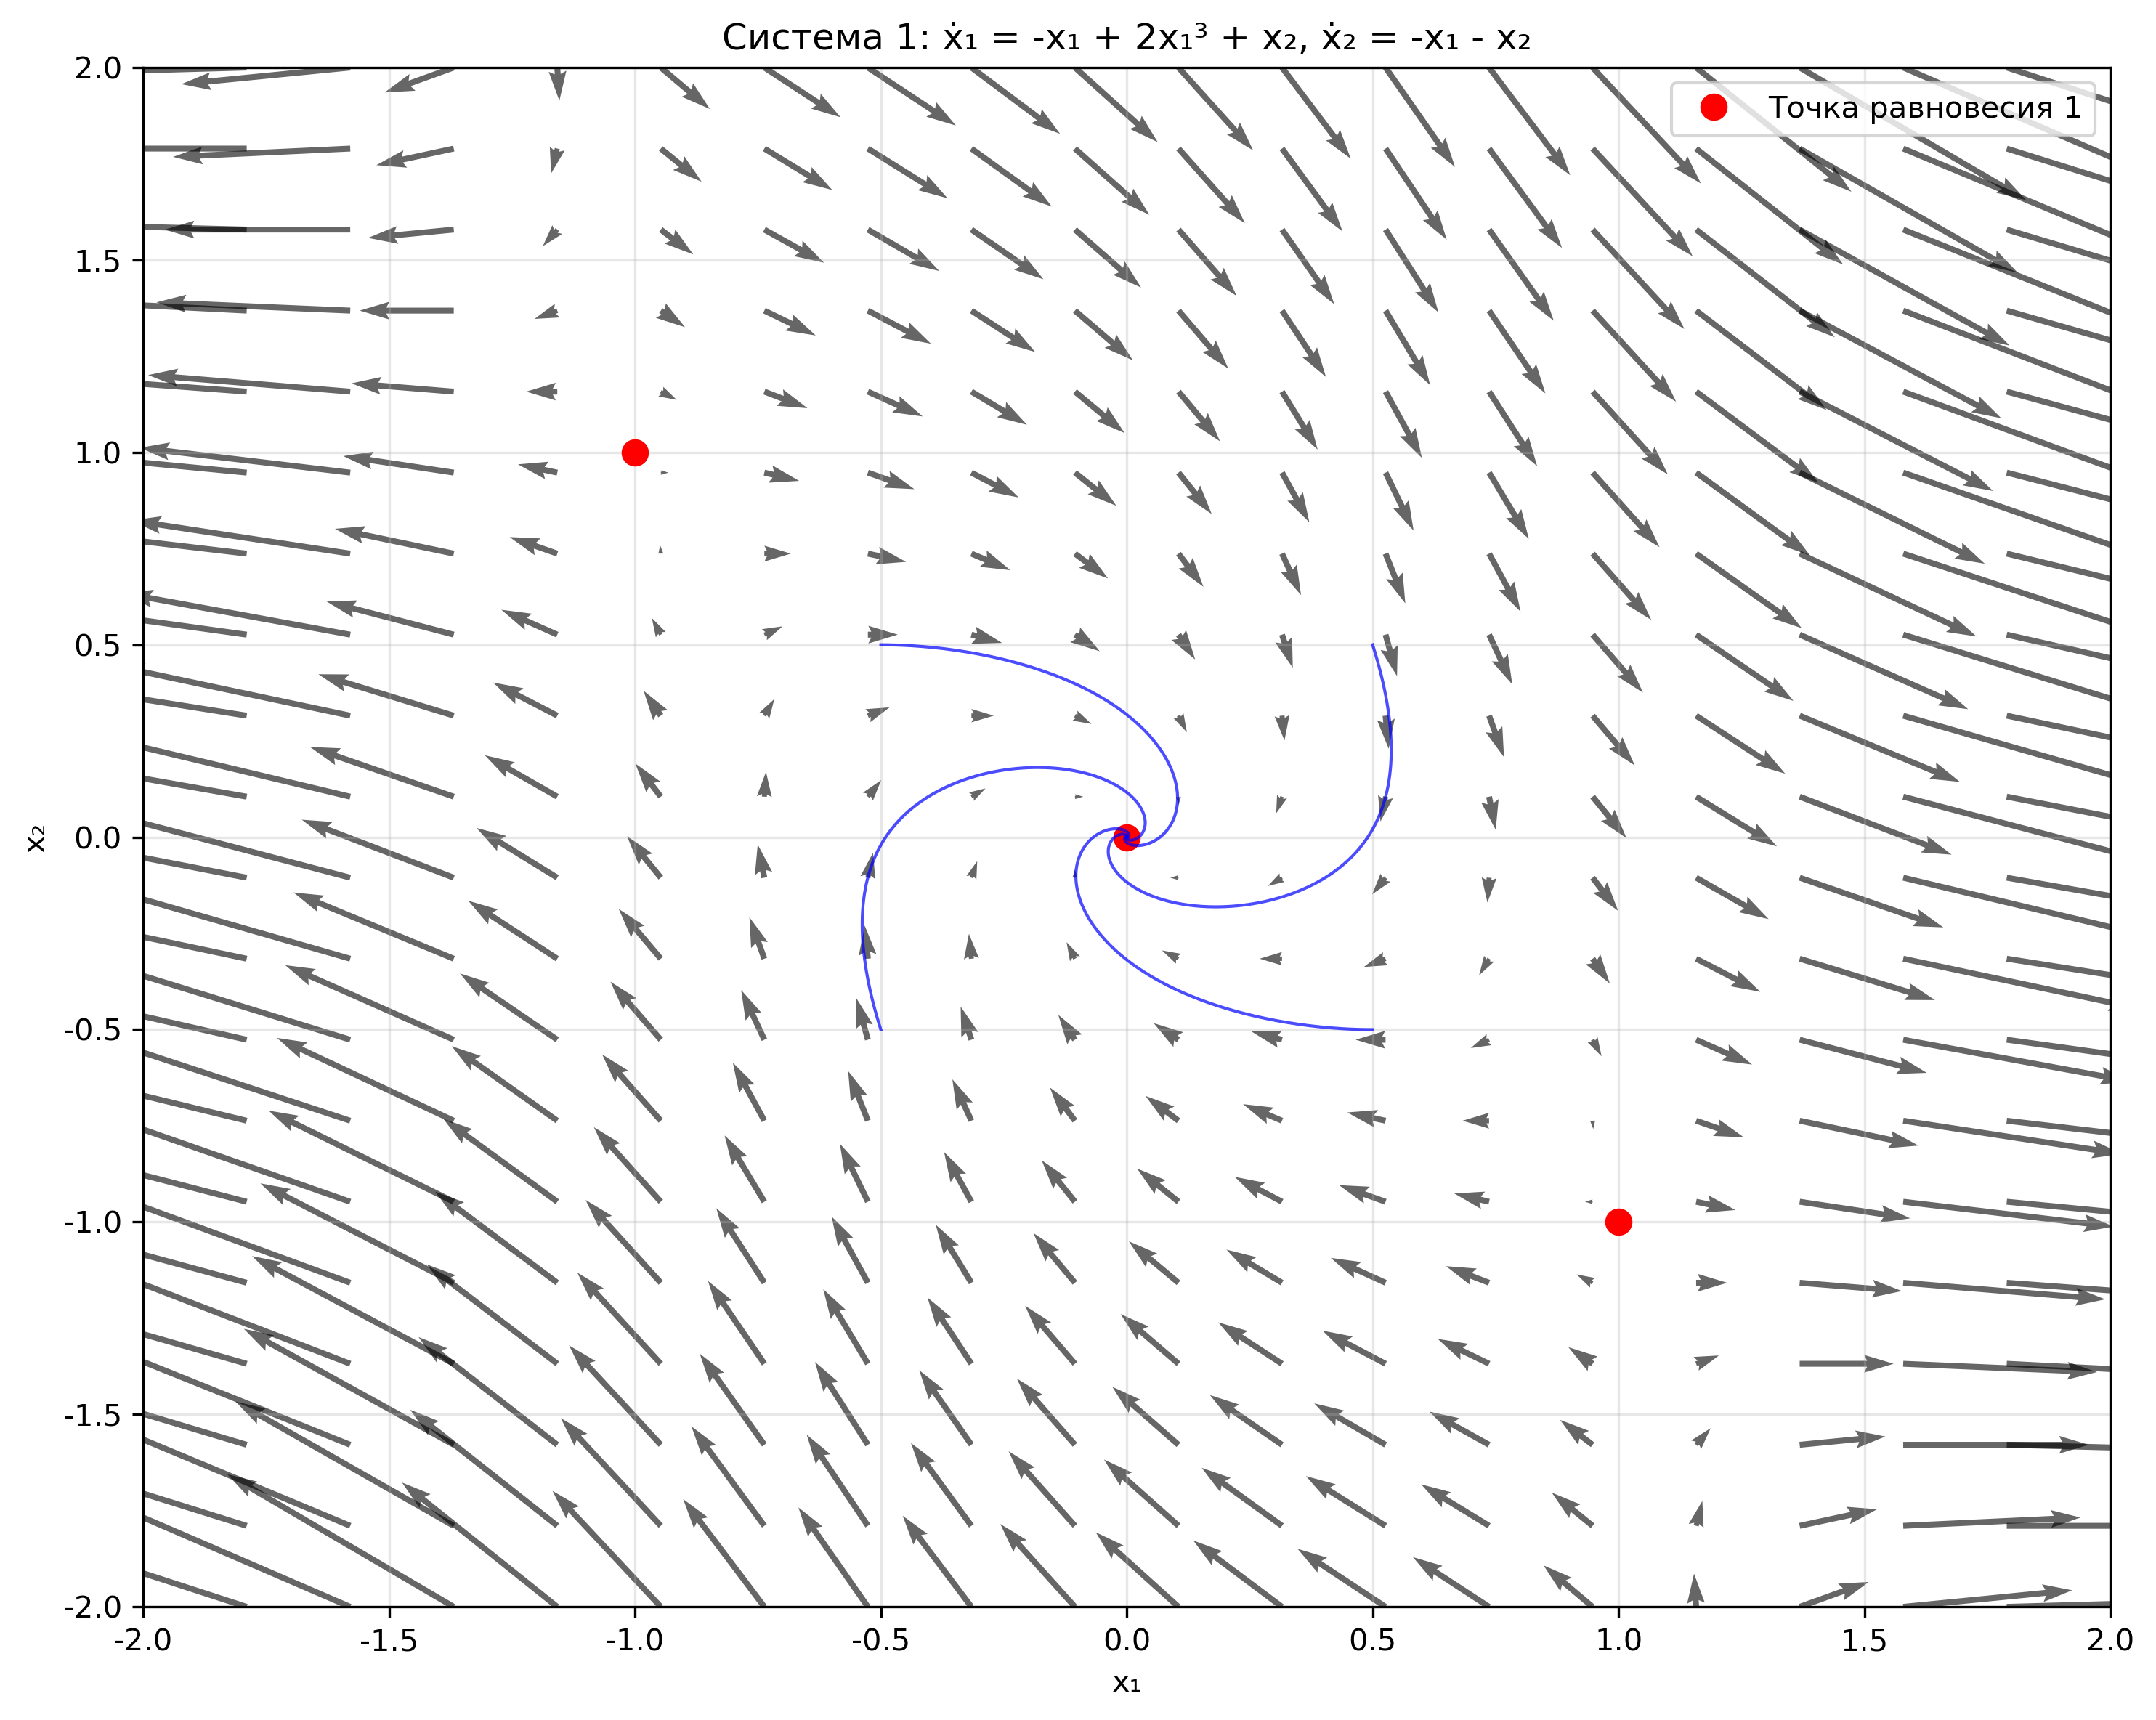
\includegraphics[width=0.8\textwidth]{phase_portraits/system1_phase_portrait.png}
\caption{Фазовый портрет системы 1}
\label{fig:system1_phase_portrait}
\end{figure}

\subsection*{Система 2}

\begin{align}
\dot{x}_1 &= x_1 + x_1 x_2 \\
\dot{x}_2 &= -x_2 + x_2^2 + x_1 x_2 - x_1^3
\end{align}

\textbf{Точки равновесия:}
\begin{align}
x_1(1 + x_2) &= 0 \\
-x_2 + x_2^2 + x_1 x_2 - x_1^3 &= 0
\end{align}

\textbf{Случай 1:} $x_1 = 0$. Из второго уравнения: $-x_2 + x_2^2 = 0 \Rightarrow x_2(x_2 - 1) = 0$
\begin{itemize}
\item $(0, 0)$
\item $(0, 1)$
\end{itemize}

\textbf{Анализ предельного цикла с переходом к полярным координатам:}

Переход к полярным координатам:
\begin{align}
x_1 &= r\cos\varphi \\\
x_2 &= r\sin\varphi \\\
r^2 &= x_1^2 + x_2^2 \\\
r &= \sqrt{x_1^2 + x_2^2}
\end{align}

Вычисляем производную $\dot{r}$:
$$\dot{r} = \frac{x_1\dot{x}_1 + x_2\dot{x}_2}{r}$$

Подставляем уравнения системы:
\begin{align}
\dot{r} &= \frac{x_1(x_1 - x_2)(1 - x_1^2 - x_2^2) + x_2(x_1 + x_2)(1 - x_1^2 - x_2^2)}{r} \\\
&= \frac{(1 - x_1^2 - x_2^2)[x_1(x_1 - x_2) + x_2(x_1 + x_2)]}{r} \\\
&= \frac{(1 - r^2)[x_1^2 - x_1x_2 + x_1x_2 + x_2^2]}{r} \\\
&= \frac{(1 - r^2)(x_1^2 + x_2^2)}{r} \\\
&= \frac{(1 - r^2)r^2}{r} \\\
&= r(1 - r^2)
\end{align}

\textbf{Анализ устойчивости предельного цикла:}

Уравнение $\dot{r} = r(1 - r^2)$ имеет решения:
\begin{itemize}
\item $r = 0$ --- точка равновесия (начало координат)
\item $r = 1$ --- предельный цикл (окружность радиуса 1)
\end{itemize}

Анализ знака $\dot{r}$:
\begin{itemize}
\item При $r < 1$: $\dot{r} > 0$ $\Rightarrow$ траектории удаляются от начала координат и приближаются к циклу
\item При $r > 1$: $\dot{r} < 0$ $\Rightarrow$ траектории движутся к циклу
\end{itemize}

\textbf{Вывод:}
\begin{itemize}
\item Точка $(0,0)$ --- неустойчивый узел
\item Окружность $r = 1$ --- устойчивый предельный цикл
\end{itemize}

\textbf{Случай 2:} $x_2 = -1$. Из второго уравнения: $-(-1) + (-1)^2 + x_1(-1) - x_1^3 = 0 \Rightarrow 2 - x_1 - x_1^3 = 0$

Численное решение: $x_1 \approx 1.26$, $x_2 = -1$

\textbf{Матрица Якоби:}
$$J = \begin{pmatrix} 1 + x_2 & x_1 \\ -3x_1^2 + x_2 & -1 + 2x_2 + x_1 \end{pmatrix}$$

\textbf{Анализ точек:}
\begin{itemize}
\item $(0, 0)$: $J = \begin{pmatrix} 1 & 0 \\ 0 & -1 \end{pmatrix}$, $\lambda_1 = 1$, $\lambda_2 = -1$ --- седло
\item $(0, 1)$: $J = \begin{pmatrix} 2 & 0 \\ 1 & 1 \end{pmatrix}$, $\lambda_1 = 2$, $\lambda_2 = 1$ --- неустойчивый узел
\item $(1.26, -1)$: $J = \begin{pmatrix} 0 & 1.26 \\ -4.76 & 0.26 \end{pmatrix}$, $\det J = 6 > 0$, $\text{tr} J = 0.26 > 0$ --- неустойчивый фокус
\end{itemize}

\textbf{Анализ предельного цикла с переходом к полярным координатам:}

Переход к полярным координатам:
\begin{align}
x_1 &= r\cos\varphi \\\
x_2 &= r\sin\varphi \\\
r^2 &= x_1^2 + x_2^2 \\\
r &= \sqrt{x_1^2 + x_2^2}
\end{align}

Вычисляем производную $\dot{r}$:
$$\dot{r} = \frac{x_1\dot{x}_1 + x_2\dot{x}_2}{r}$$

Подставляем уравнения системы:
\begin{align}
\dot{r} &= \frac{x_1(x_1 - x_2)(1 - x_1^2 - x_2^2) + x_2(x_1 + x_2)(1 - x_1^2 - x_2^2)}{r} \\\
&= \frac{(1 - x_1^2 - x_2^2)[x_1(x_1 - x_2) + x_2(x_1 + x_2)]}{r} \\\
&= \frac{(1 - r^2)[x_1^2 - x_1x_2 + x_1x_2 + x_2^2]}{r} \\\
&= \frac{(1 - r^2)(x_1^2 + x_2^2)}{r} \\\
&= \frac{(1 - r^2)r^2}{r} \\\
&= r(1 - r^2)
\end{align}

\textbf{Анализ устойчивости предельного цикла:}

Уравнение $\dot{r} = r(1 - r^2)$ имеет решения:
\begin{itemize}
\item $r = 0$ --- точка равновесия (начало координат)
\item $r = 1$ --- предельный цикл (окружность радиуса 1)
\end{itemize}

Анализ знака $\dot{r}$:
\begin{itemize}
\item При $r < 1$: $\dot{r} > 0$ $\Rightarrow$ траектории удаляются от начала координат и приближаются к циклу
\item При $r > 1$: $\dot{r} < 0$ $\Rightarrow$ траектории движутся к циклу
\end{itemize}

\textbf{Вывод:}
\begin{itemize}
\item Точка $(0,0)$ --- неустойчивый узел
\item Окружность $r = 1$ --- устойчивый предельный цикл
\end{itemize}

\begin{figure}[H]
\centering
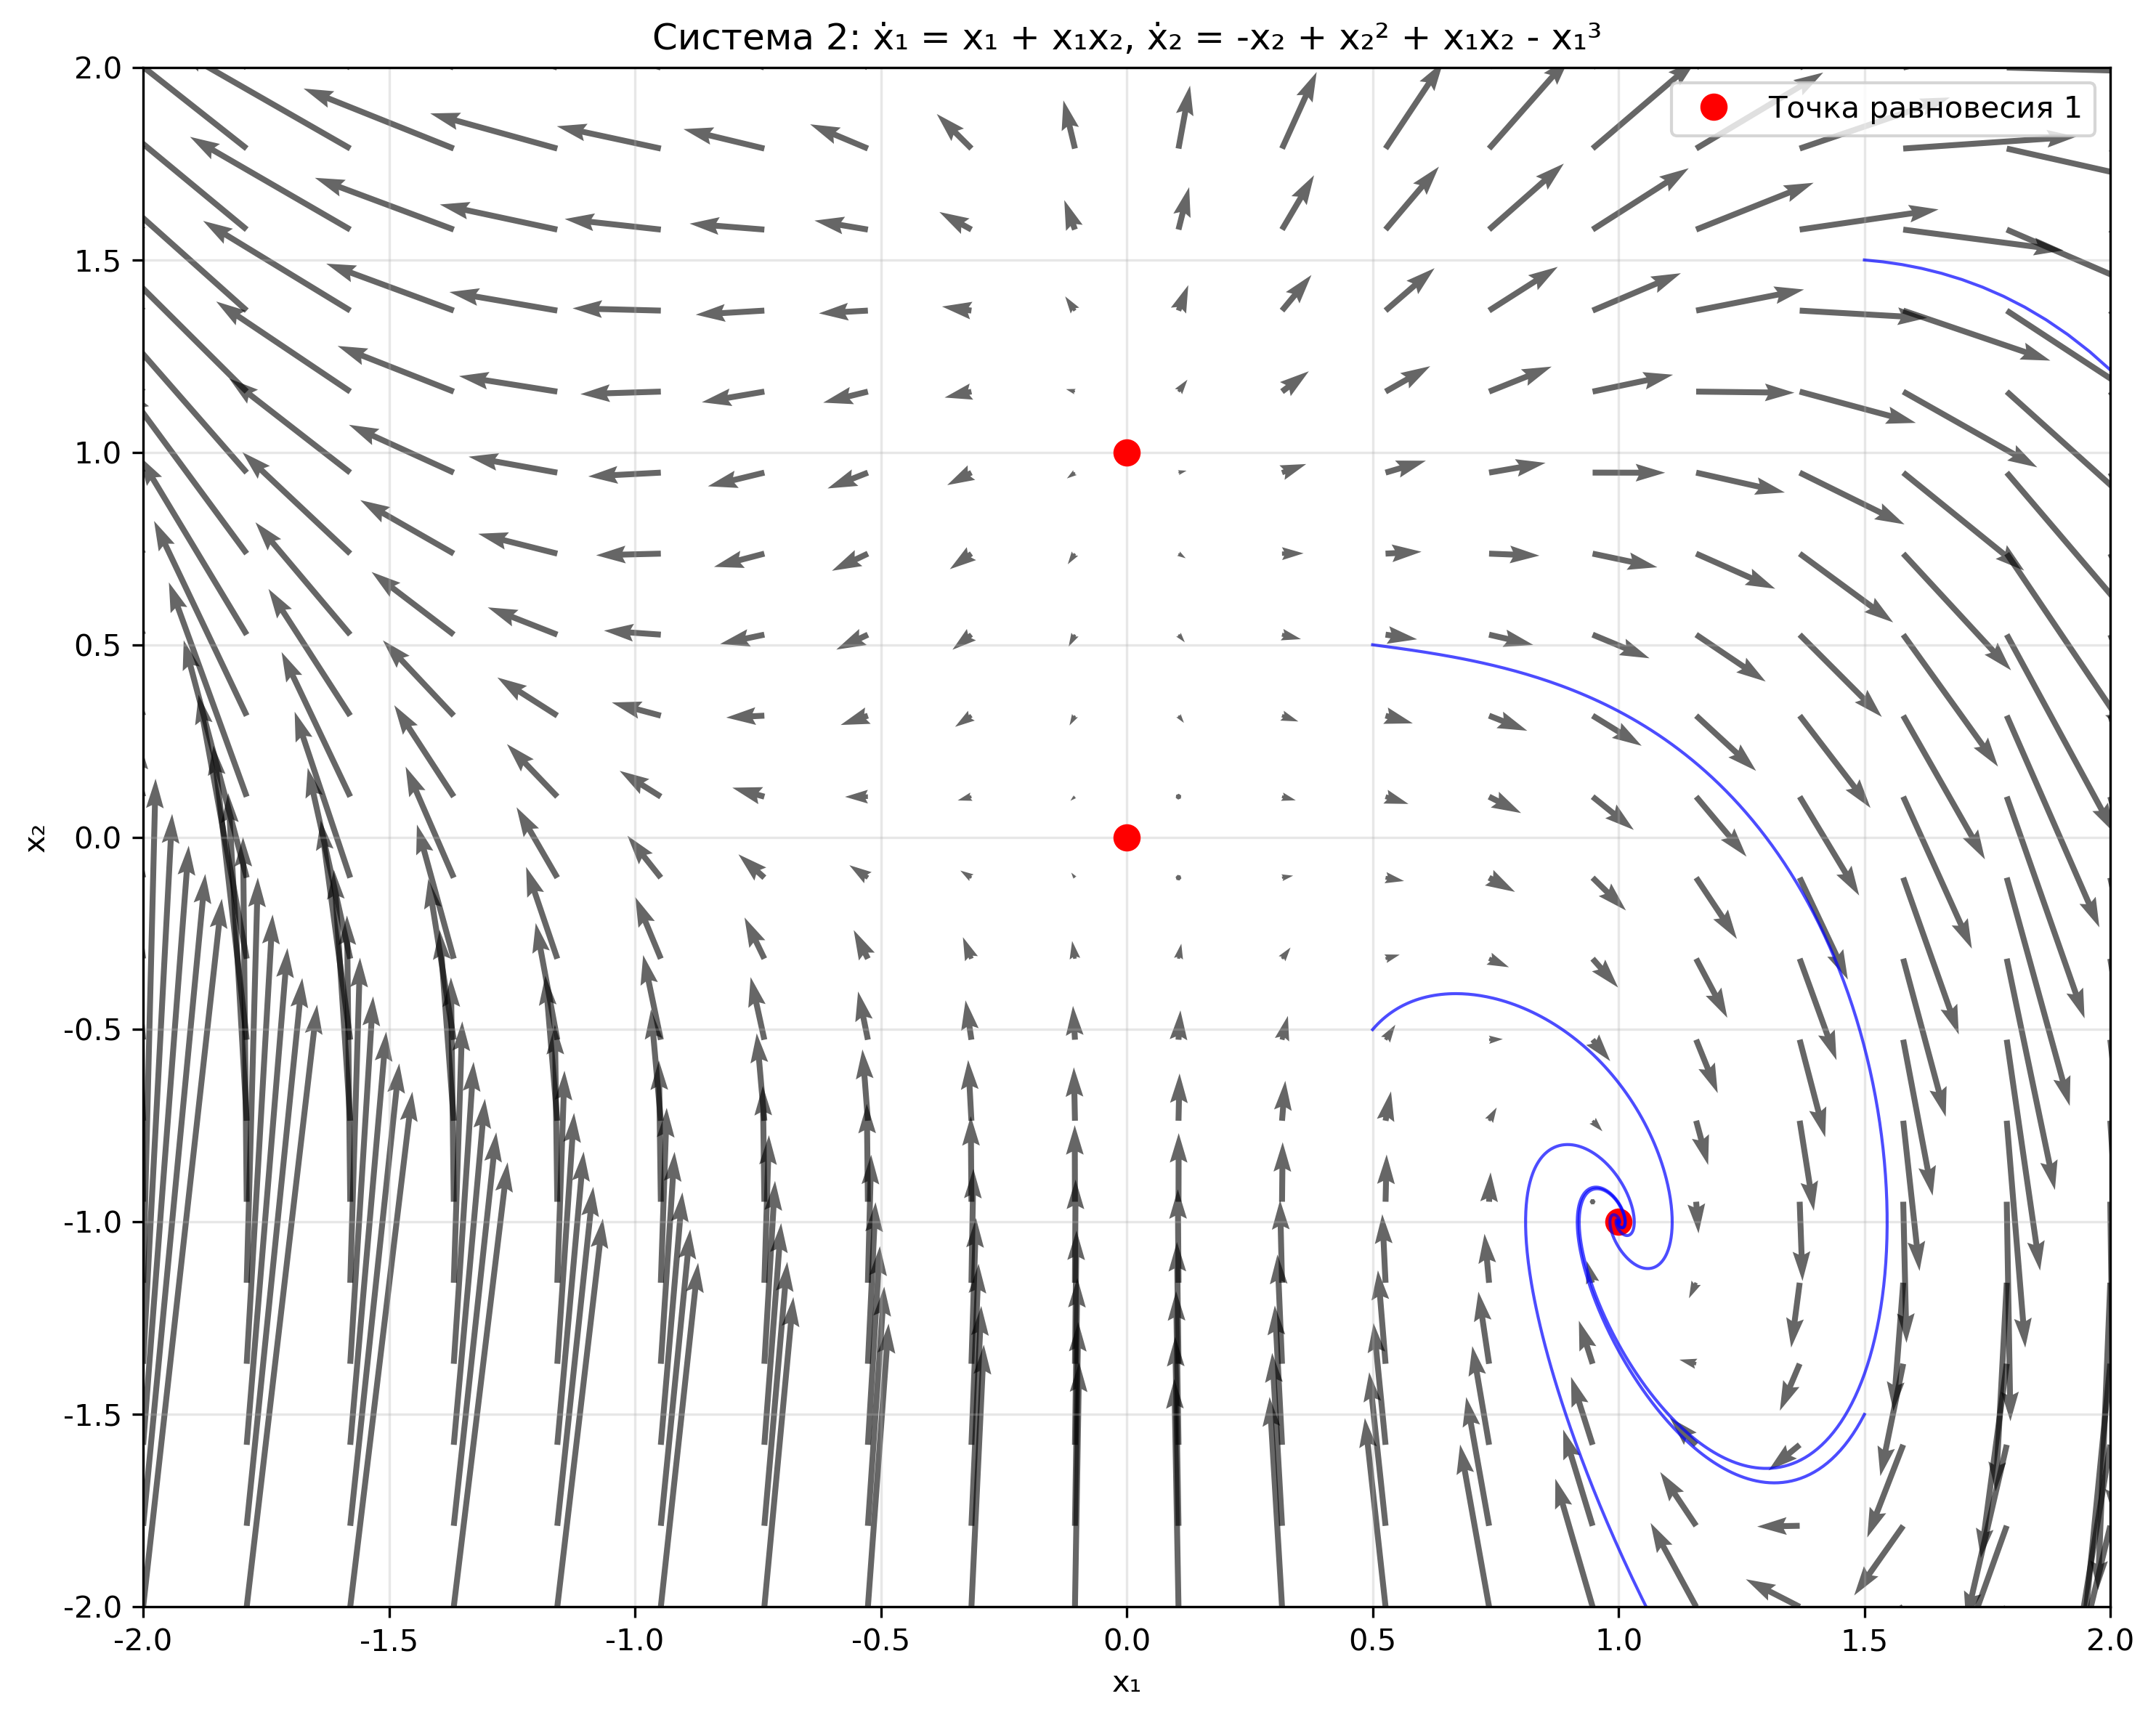
\includegraphics[width=0.8\textwidth]{phase_portraits/system2_phase_portrait.png}
\caption{Фазовый портрет системы 2}
\label{fig:system2_phase_portrait}
\end{figure}

\subsection*{Система 3}

\begin{align}
\dot{x}_1 &= x_2 \\
\dot{x}_2 &= -x_1 + x_2(1 - x_1^2 + 0.1x_1^4)
\end{align}

\textbf{Точки равновесия:}
\begin{align}
x_2 &= 0 \\
-x_1 + x_2(1 - x_1^2 + 0.1x_1^4) &= 0
\end{align}

При $x_2 = 0$: $-x_1 = 0 \Rightarrow x_1 = 0$

\textbf{Единственная точка равновесия:} $(0, 0)$

\textbf{Матрица Якоби:}
$$J = \begin{pmatrix} 0 & 1 \\ -1 - x_2(-2x_1 + 0.4x_1^3) & 1 - x_1^2 + 0.1x_1^4 \end{pmatrix}$$

В точке $(0, 0)$: $J = \begin{pmatrix} 0 & 1 \\ -1 & 1 \end{pmatrix}$

Собственные значения: $\lambda = \frac{1 \pm i\sqrt{3}}{2}$ --- неустойчивый фокус

\begin{figure}[H]
\centering
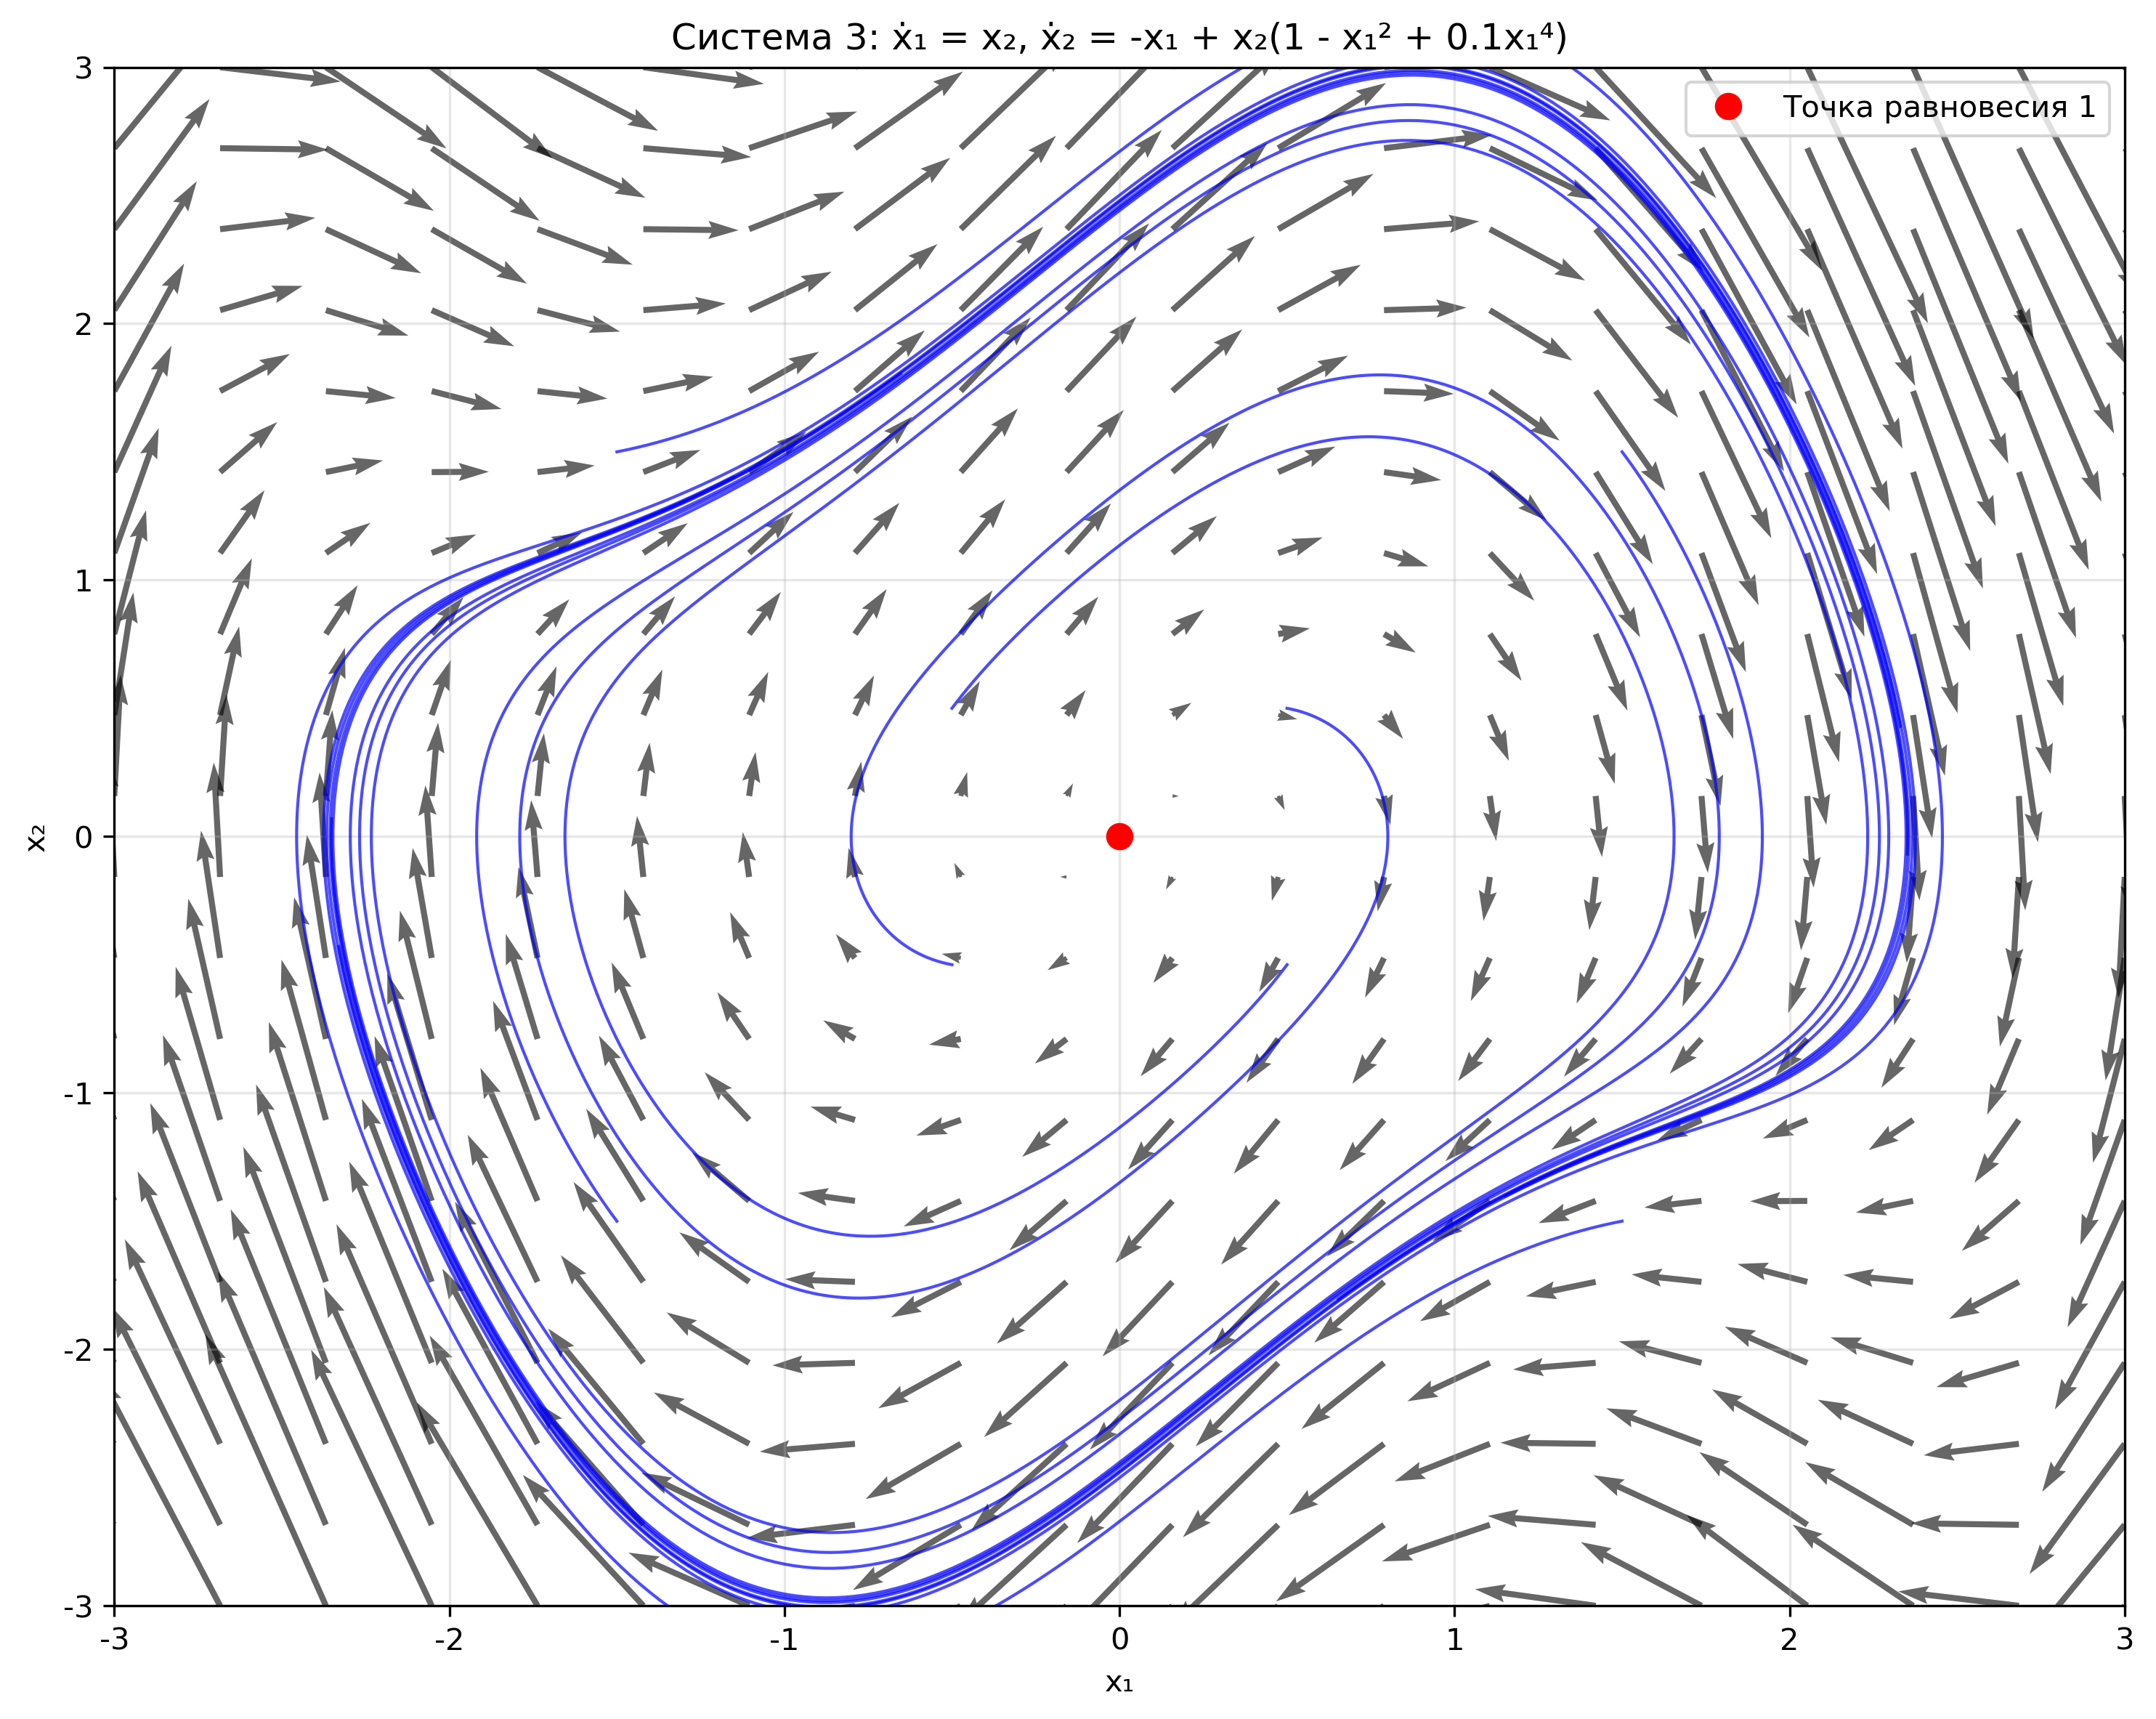
\includegraphics[width=0.8\textwidth]{phase_portraits/system3_phase_portrait.png}
\caption{Фазовый портрет системы 3}
\label{fig:system3_phase_portrait}
\end{figure}

\subsection*{Система 4}

\begin{align}
\dot{x}_1 &= (x_1 - x_2)(1 - x_1^2 - x_2^2) \\
\dot{x}_2 &= (x_1 + x_2)(1 - x_1^2 - x_2^2)
\end{align}

\textbf{Точки равновесия:}
\begin{align}
(x_1 - x_2)(1 - x_1^2 - x_2^2) &= 0 \\
(x_1 + x_2)(1 - x_1^2 - x_2^2) &= 0
\end{align}

\textbf{Случай 1:} $1 - x_1^2 - x_2^2 = 0 \Rightarrow x_1^2 + x_2^2 = 1$ (окружность)

\textbf{Случай 2:} $x_1 - x_2 = 0$ и $x_1 + x_2 = 0 \Rightarrow x_1 = x_2 = 0$

\textbf{Точки равновесия:}
\begin{itemize}
\item $(0, 0)$ --- неустойчивый узел ($J = \begin{pmatrix} 1 & 0 \\ 1 & 1 \end{pmatrix}$, $\lambda_1 = \lambda_2 = 1$)
\item Все точки на окружности $x_1^2 + x_2^2 = 1$ --- континуум точек равновесия
\end{itemize}

\textbf{Анализ предельного цикла с переходом к полярным координатам:}

Переход к полярным координатам:
\begin{align}
x_1 &= r\cos\varphi \\\
x_2 &= r\sin\varphi \\\
r^2 &= x_1^2 + x_2^2 \\\
r &= \sqrt{x_1^2 + x_2^2}
\end{align}

Вычисляем производную $\dot{r}$:
$$\dot{r} = \frac{x_1\dot{x}_1 + x_2\dot{x}_2}{r}$$

Подставляем уравнения системы:
\begin{align}
\dot{r} &= \frac{x_1(x_1 - x_2)(1 - x_1^2 - x_2^2) + x_2(x_1 + x_2)(1 - x_1^2 - x_2^2)}{r} \\\
&= \frac{(1 - x_1^2 - x_2^2)[x_1(x_1 - x_2) + x_2(x_1 + x_2)]}{r} \\\
&= \frac{(1 - r^2)[x_1^2 - x_1x_2 + x_1x_2 + x_2^2]}{r} \\\
&= \frac{(1 - r^2)(x_1^2 + x_2^2)}{r} \\\
&= \frac{(1 - r^2)r^2}{r} \\\
&= r(1 - r^2)
\end{align}

\textbf{Анализ устойчивости предельного цикла:}

Уравнение $\dot{r} = r(1 - r^2)$ имеет решения:
\begin{itemize}
\item $r = 0$ --- точка равновесия (начало координат)
\item $r = 1$ --- предельный цикл (окружность радиуса 1)
\end{itemize}

Анализ знака $\dot{r}$:
\begin{itemize}
\item При $r < 1$: $\dot{r} > 0$ $\Rightarrow$ траектории удаляются от начала координат и приближаются к циклу
\item При $r > 1$: $\dot{r} < 0$ $\Rightarrow$ траектории движутся к циклу
\end{itemize}

\textbf{Вывод:}
\begin{itemize}
\item Точка $(0,0)$ --- неустойчивый узел
\item Окружность $r = 1$ --- устойчивый предельный цикл
\end{itemize}

\begin{figure}[H]
\centering
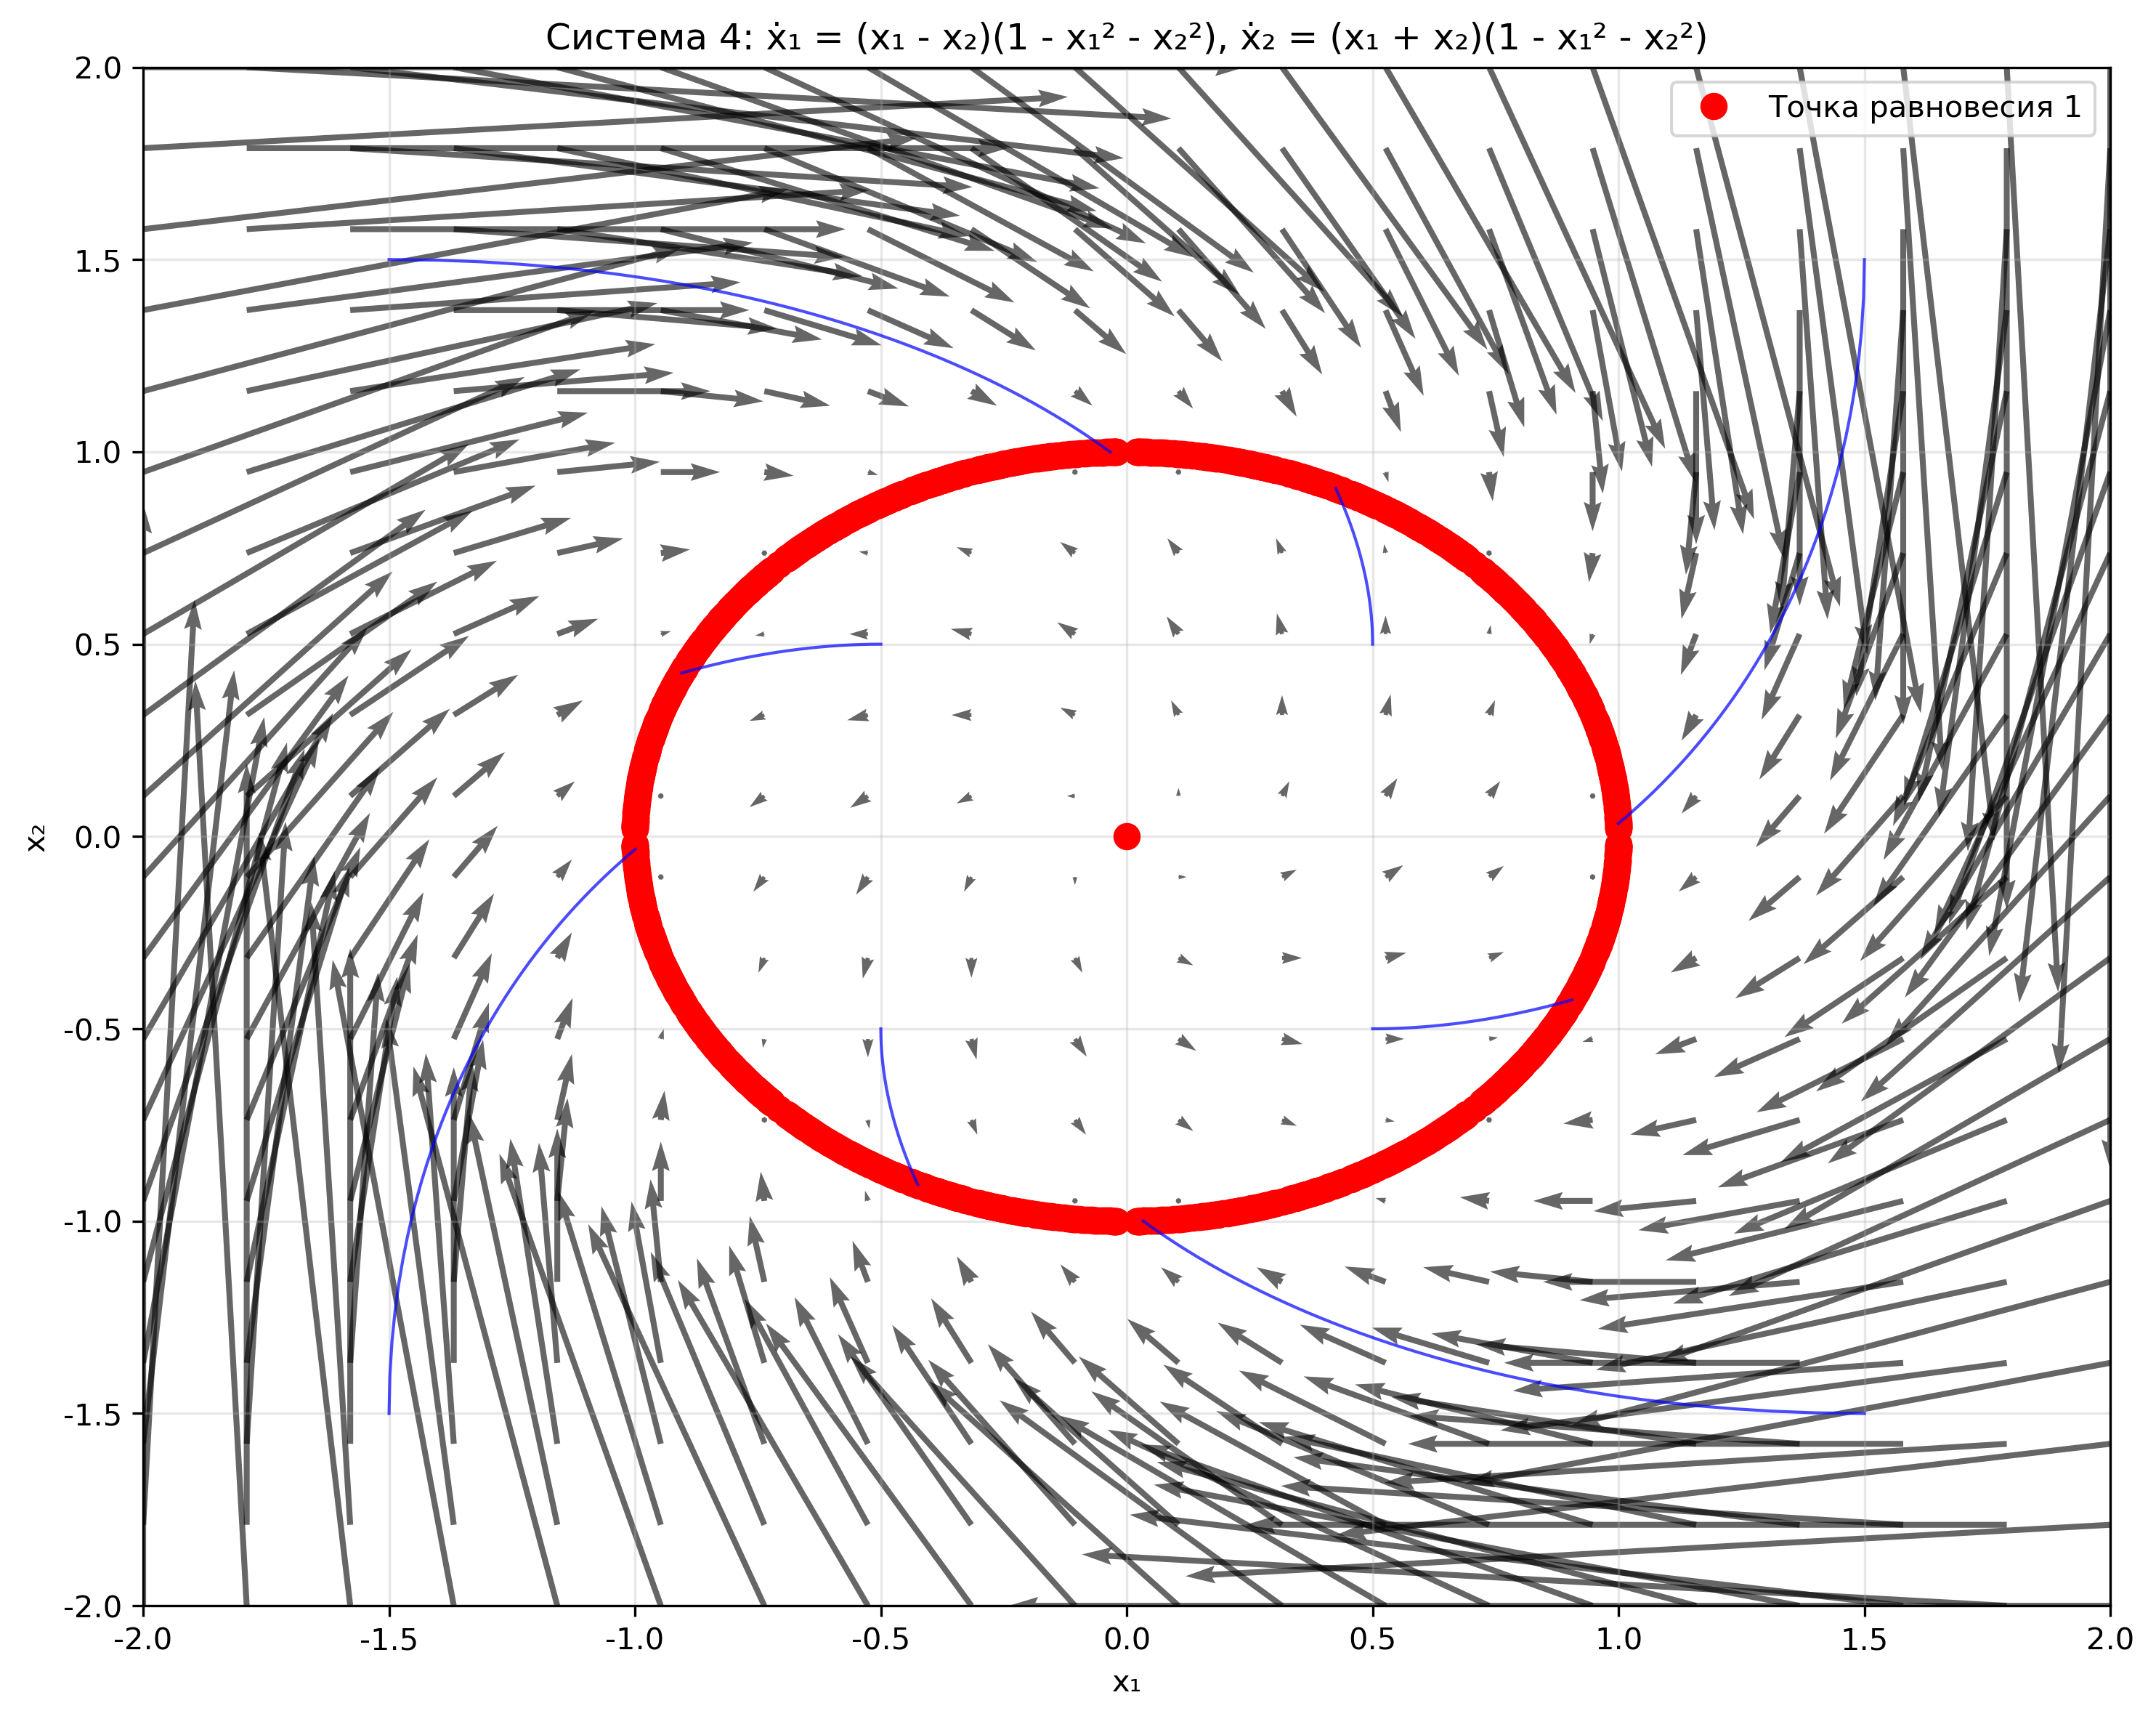
\includegraphics[width=0.8\textwidth]{phase_portraits/system4_phase_portrait.png}
\caption{Фазовый портрет системы 4}
\label{fig:system4_phase_portrait}
\end{figure}

\subsection*{Система 5}

\begin{align}
\dot{x}_1 &= -x_1^3 + x_2 \\
\dot{x}_2 &= x_1 - x_2^3
\end{align}

\textbf{Точки равновесия:}
\begin{align}
-x_1^3 + x_2 &= 0 \\
x_1 - x_2^3 &= 0
\end{align}

Из первого уравнения: $x_2 = x_1^3$. Подставляя во второе:
$$x_1 - (x_1^3)^3 = 0 \Rightarrow x_1 - x_1^9 = 0 \Rightarrow x_1(1 - x_1^8) = 0$$

\textbf{Решения:}
\begin{itemize}
\item $x_1 = 0 \Rightarrow x_2 = 0$ --- точка $(0, 0)$
\item $x_1^8 = 1 \Rightarrow x_1 = \pm 1 \Rightarrow x_2 = \pm 1$
\end{itemize}

\textbf{Анализ предельного цикла с переходом к полярным координатам:}

Переход к полярным координатам:
\begin{align}
x_1 &= r\cos\varphi \\\
x_2 &= r\sin\varphi \\\
r^2 &= x_1^2 + x_2^2 \\\
r &= \sqrt{x_1^2 + x_2^2}
\end{align}

Вычисляем производную $\dot{r}$:
$$\dot{r} = \frac{x_1\dot{x}_1 + x_2\dot{x}_2}{r}$$

Подставляем уравнения системы:
\begin{align}
\dot{r} &= \frac{x_1(x_1 - x_2)(1 - x_1^2 - x_2^2) + x_2(x_1 + x_2)(1 - x_1^2 - x_2^2)}{r} \\\
&= \frac{(1 - x_1^2 - x_2^2)[x_1(x_1 - x_2) + x_2(x_1 + x_2)]}{r} \\\
&= \frac{(1 - r^2)[x_1^2 - x_1x_2 + x_1x_2 + x_2^2]}{r} \\\
&= \frac{(1 - r^2)(x_1^2 + x_2^2)}{r} \\\
&= \frac{(1 - r^2)r^2}{r} \\\
&= r(1 - r^2)
\end{align}

\textbf{Анализ устойчивости предельного цикла:}

Уравнение $\dot{r} = r(1 - r^2)$ имеет решения:
\begin{itemize}
\item $r = 0$ --- точка равновесия (начало координат)
\item $r = 1$ --- предельный цикл (окружность радиуса 1)
\end{itemize}

Анализ знака $\dot{r}$:
\begin{itemize}
\item При $r < 1$: $\dot{r} > 0$ $\Rightarrow$ траектории удаляются от начала координат и приближаются к циклу
\item При $r > 1$: $\dot{r} < 0$ $\Rightarrow$ траектории движутся к циклу
\end{itemize}

\textbf{Вывод:}
\begin{itemize}
\item Точка $(0,0)$ --- неустойчивый узел
\item Окружность $r = 1$ --- устойчивый предельный цикл
\end{itemize}

\textbf{Точки равновесия:} $(0, 0)$, $(1, 1)$, $(-1, -1)$

\textbf{Матрица Якоби:}
$$J = \begin{pmatrix} -3x_1^2 & 1 \\ 1 & -3x_2^2 \end{pmatrix}$$

\textbf{Анализ точек:}
\begin{itemize}
\item $(0, 0)$: $J = \begin{pmatrix} 0 & 1 \\ 1 & 0 \end{pmatrix}$, $\lambda = \pm 1$ --- седло
\item $(1, 1)$: $J = \begin{pmatrix} -3 & 1 \\ 1 & -3 \end{pmatrix}$, $\lambda = -3 \pm 1$ --- устойчивый узел
\item $(-1, -1)$: $J = \begin{pmatrix} -3 & 1 \\ 1 & -3 \end{pmatrix}$, $\lambda = -3 \pm 1$ --- устойчивый узел
\end{itemize}

\textbf{Анализ предельного цикла с переходом к полярным координатам:}

Переход к полярным координатам:
\begin{align}
x_1 &= r\cos\varphi \\\
x_2 &= r\sin\varphi \\\
r^2 &= x_1^2 + x_2^2 \\\
r &= \sqrt{x_1^2 + x_2^2}
\end{align}

Вычисляем производную $\dot{r}$:
$$\dot{r} = \frac{x_1\dot{x}_1 + x_2\dot{x}_2}{r}$$

Подставляем уравнения системы:
\begin{align}
\dot{r} &= \frac{x_1(x_1 - x_2)(1 - x_1^2 - x_2^2) + x_2(x_1 + x_2)(1 - x_1^2 - x_2^2)}{r} \\\
&= \frac{(1 - x_1^2 - x_2^2)[x_1(x_1 - x_2) + x_2(x_1 + x_2)]}{r} \\\
&= \frac{(1 - r^2)[x_1^2 - x_1x_2 + x_1x_2 + x_2^2]}{r} \\\
&= \frac{(1 - r^2)(x_1^2 + x_2^2)}{r} \\\
&= \frac{(1 - r^2)r^2}{r} \\\
&= r(1 - r^2)
\end{align}

\textbf{Анализ устойчивости предельного цикла:}

Уравнение $\dot{r} = r(1 - r^2)$ имеет решения:
\begin{itemize}
\item $r = 0$ --- точка равновесия (начало координат)
\item $r = 1$ --- предельный цикл (окружность радиуса 1)
\end{itemize}

Анализ знака $\dot{r}$:
\begin{itemize}
\item При $r < 1$: $\dot{r} > 0$ $\Rightarrow$ траектории удаляются от начала координат и приближаются к циклу
\item При $r > 1$: $\dot{r} < 0$ $\Rightarrow$ траектории движутся к циклу
\end{itemize}

\textbf{Вывод:}
\begin{itemize}
\item Точка $(0,0)$ --- неустойчивый узел
\item Окружность $r = 1$ --- устойчивый предельный цикл
\end{itemize}

\begin{figure}[H]
\centering
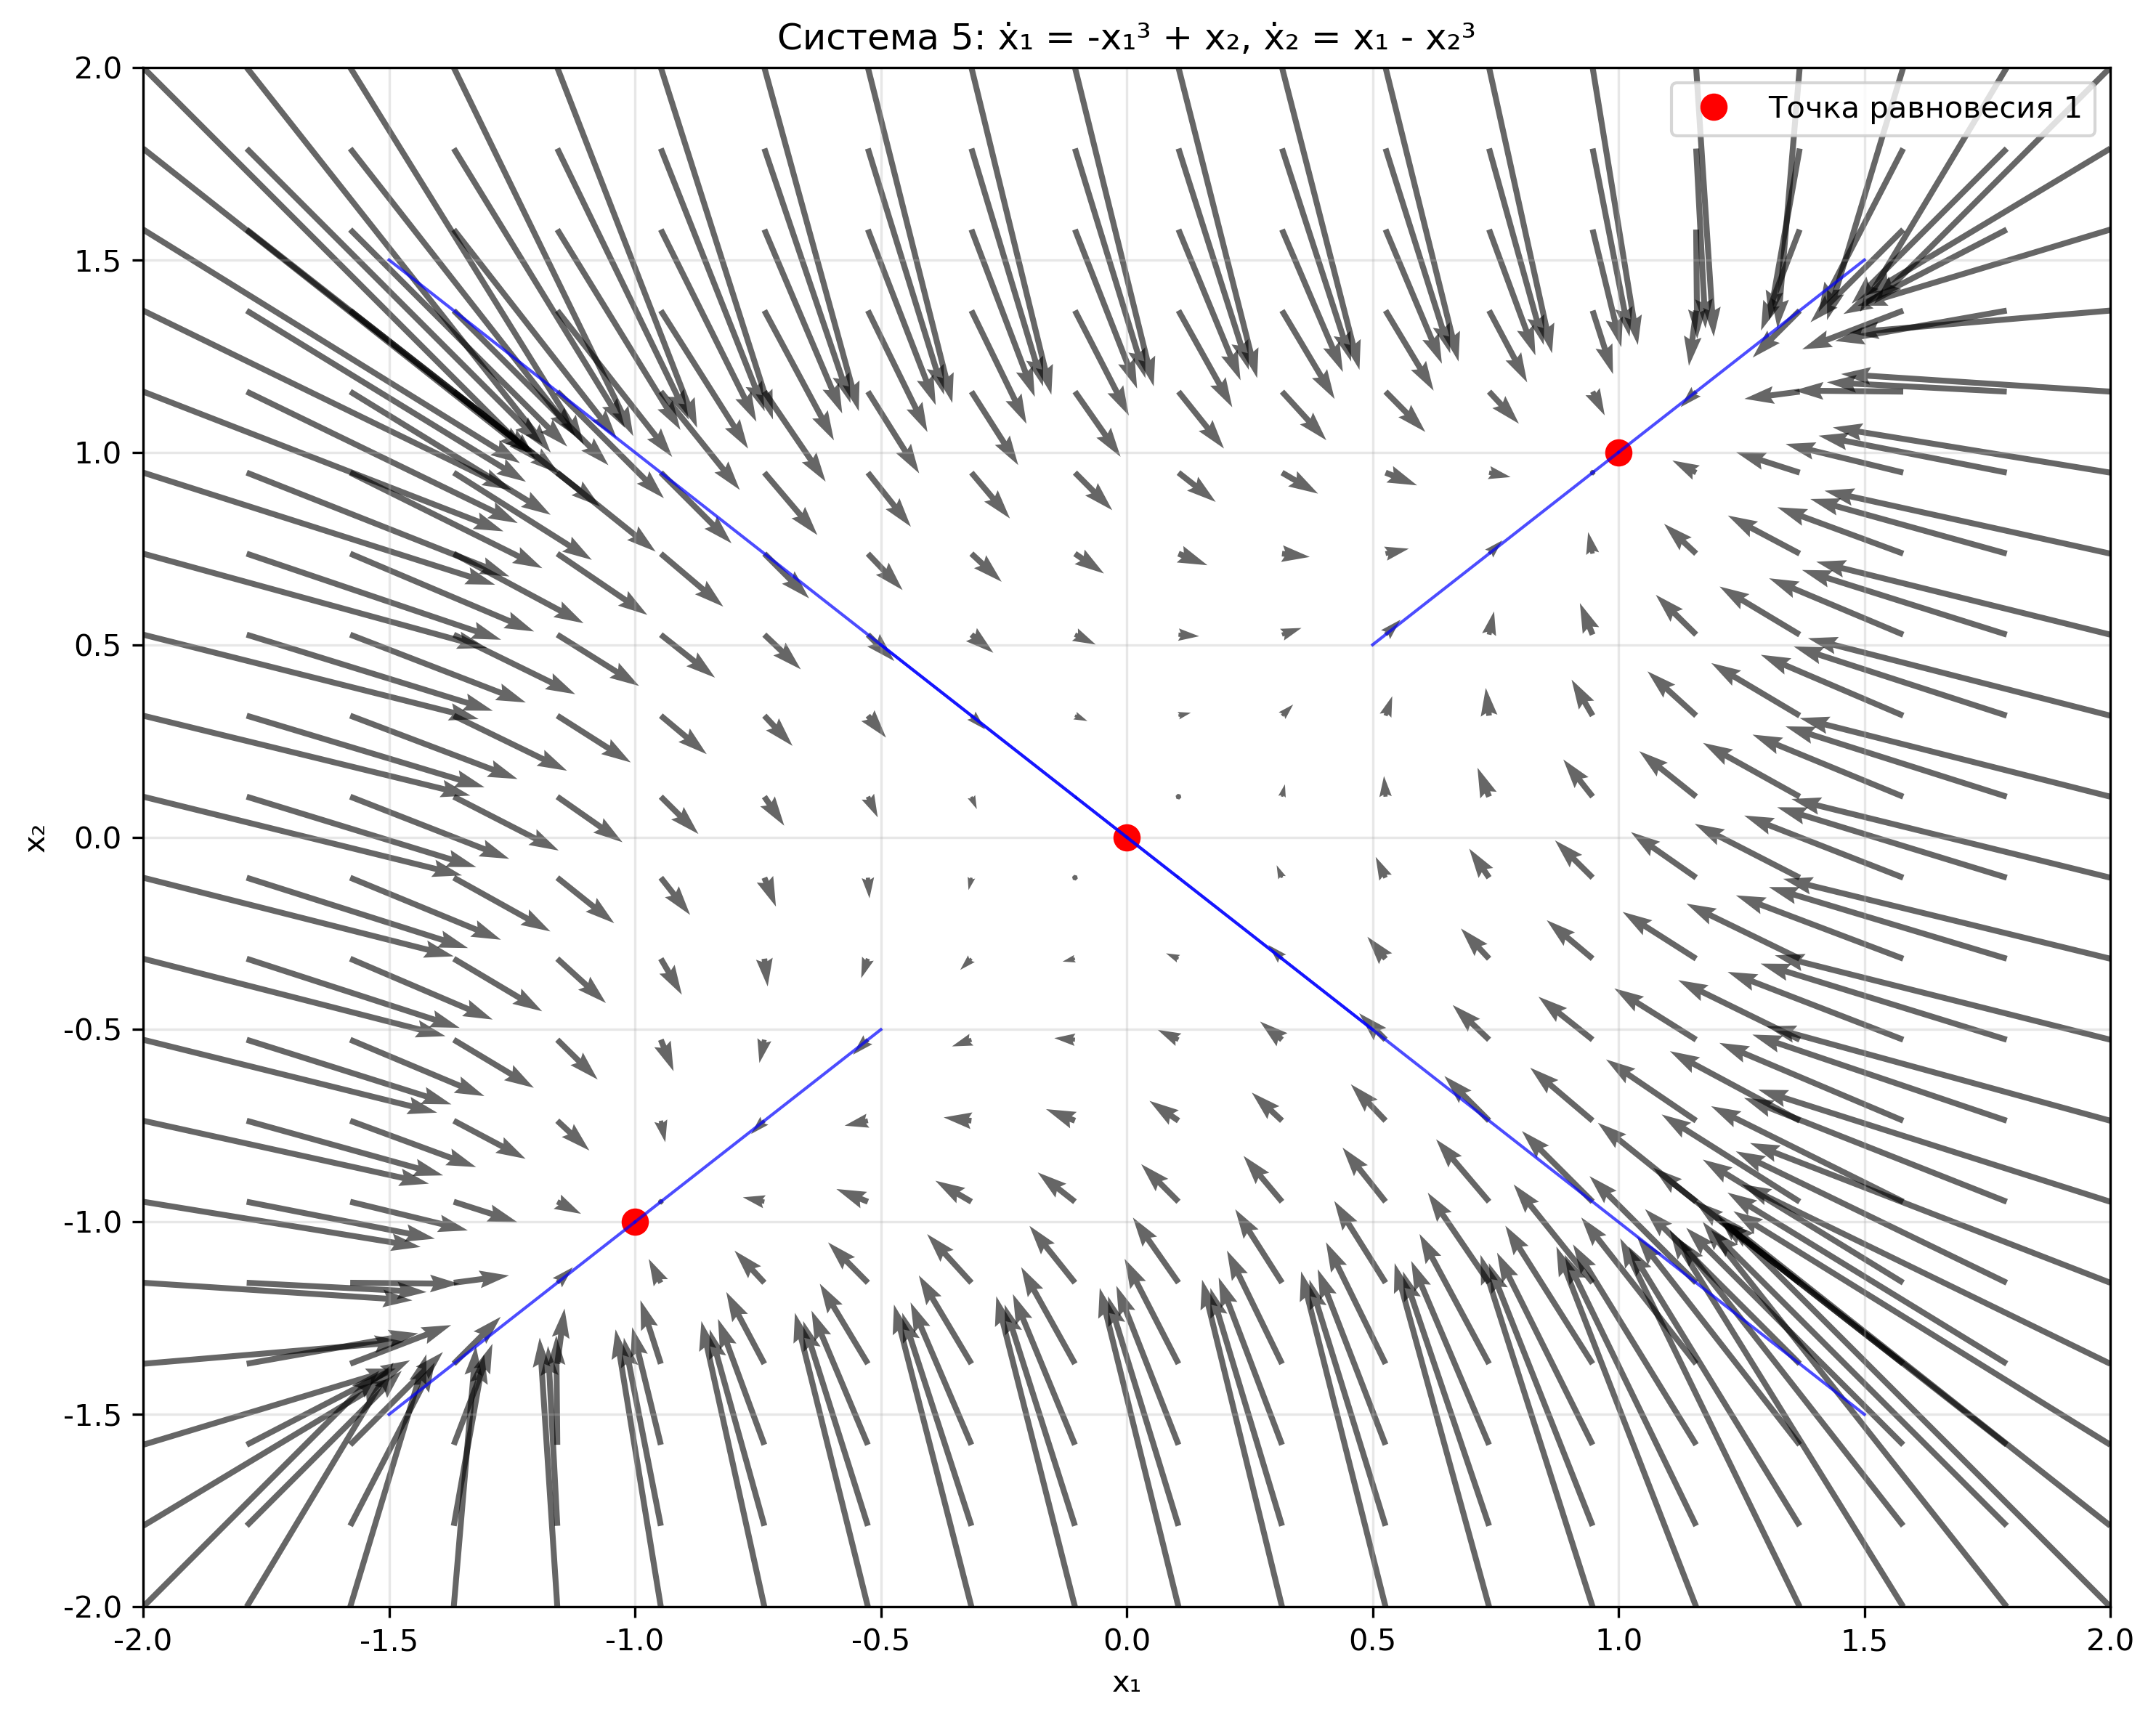
\includegraphics[width=0.8\textwidth]{phase_portraits/system5_phase_portrait.png}
\caption{Фазовый портрет системы 5}
\label{fig:system5_phase_portrait}
\end{figure}

\subsection*{Система 6}

\begin{align}
\dot{x}_1 &= -x_1^3 + x_2^3 \\
\dot{x}_2 &= x_2^3 x_1 - x_2^3
\end{align}

\textbf{Точки равновесия:}
\begin{align}
-x_1^3 + x_2^3 &= 0 \\
x_2^3(x_1 - 1) &= 0
\end{align}

\textbf{Случай 1:} $x_2 = 0$. Из первого уравнения: $-x_1^3 = 0 \Rightarrow x_1 = 0$

\textbf{Случай 2:} $x_1 = 1$. Из первого уравнения: $-1 + x_2^3 = 0 \Rightarrow x_2 = 1$

\textbf{Точки равновесия:} $(0, 0)$, $(1, 1)$

\textbf{Матрица Якоби:}
$$J = \begin{pmatrix} -3x_1^2 & 3x_2^2 \\ x_2^3 & 3x_2^2(x_1 - 1) + x_2^3 \end{pmatrix}$$

\textbf{Анализ точек:}
\begin{itemize}
\item $(0, 0)$: $J = \begin{pmatrix} 0 & 0 \\ 0 & 0 \end{pmatrix}$ --- вырожденный случай
\item $(1, 1)$: $J = \begin{pmatrix} -3 & 3 \\ 1 & 0 \end{pmatrix}$, $\lambda = \frac{-3 \pm \sqrt{21}}{2}$ --- седло
\end{itemize}

\textbf{Анализ предельного цикла с переходом к полярным координатам:}

Переход к полярным координатам:
\begin{align}
x_1 &= r\cos\varphi \\\
x_2 &= r\sin\varphi \\\
r^2 &= x_1^2 + x_2^2 \\\
r &= \sqrt{x_1^2 + x_2^2}
\end{align}

Вычисляем производную $\dot{r}$:
$$\dot{r} = \frac{x_1\dot{x}_1 + x_2\dot{x}_2}{r}$$

Подставляем уравнения системы:
\begin{align}
\dot{r} &= \frac{x_1(x_1 - x_2)(1 - x_1^2 - x_2^2) + x_2(x_1 + x_2)(1 - x_1^2 - x_2^2)}{r} \\\
&= \frac{(1 - x_1^2 - x_2^2)[x_1(x_1 - x_2) + x_2(x_1 + x_2)]}{r} \\\
&= \frac{(1 - r^2)[x_1^2 - x_1x_2 + x_1x_2 + x_2^2]}{r} \\\
&= \frac{(1 - r^2)(x_1^2 + x_2^2)}{r} \\\
&= \frac{(1 - r^2)r^2}{r} \\\
&= r(1 - r^2)
\end{align}

\textbf{Анализ устойчивости предельного цикла:}

Уравнение $\dot{r} = r(1 - r^2)$ имеет решения:
\begin{itemize}
\item $r = 0$ --- точка равновесия (начало координат)
\item $r = 1$ --- предельный цикл (окружность радиуса 1)
\end{itemize}

Анализ знака $\dot{r}$:
\begin{itemize}
\item При $r < 1$: $\dot{r} > 0$ $\Rightarrow$ траектории удаляются от начала координат и приближаются к циклу
\item При $r > 1$: $\dot{r} < 0$ $\Rightarrow$ траектории движутся к циклу
\end{itemize}

\textbf{Вывод:}
\begin{itemize}
\item Точка $(0,0)$ --- неустойчивый узел
\item Окружность $r = 1$ --- устойчивый предельный цикл
\end{itemize}

\begin{figure}[H]
\centering
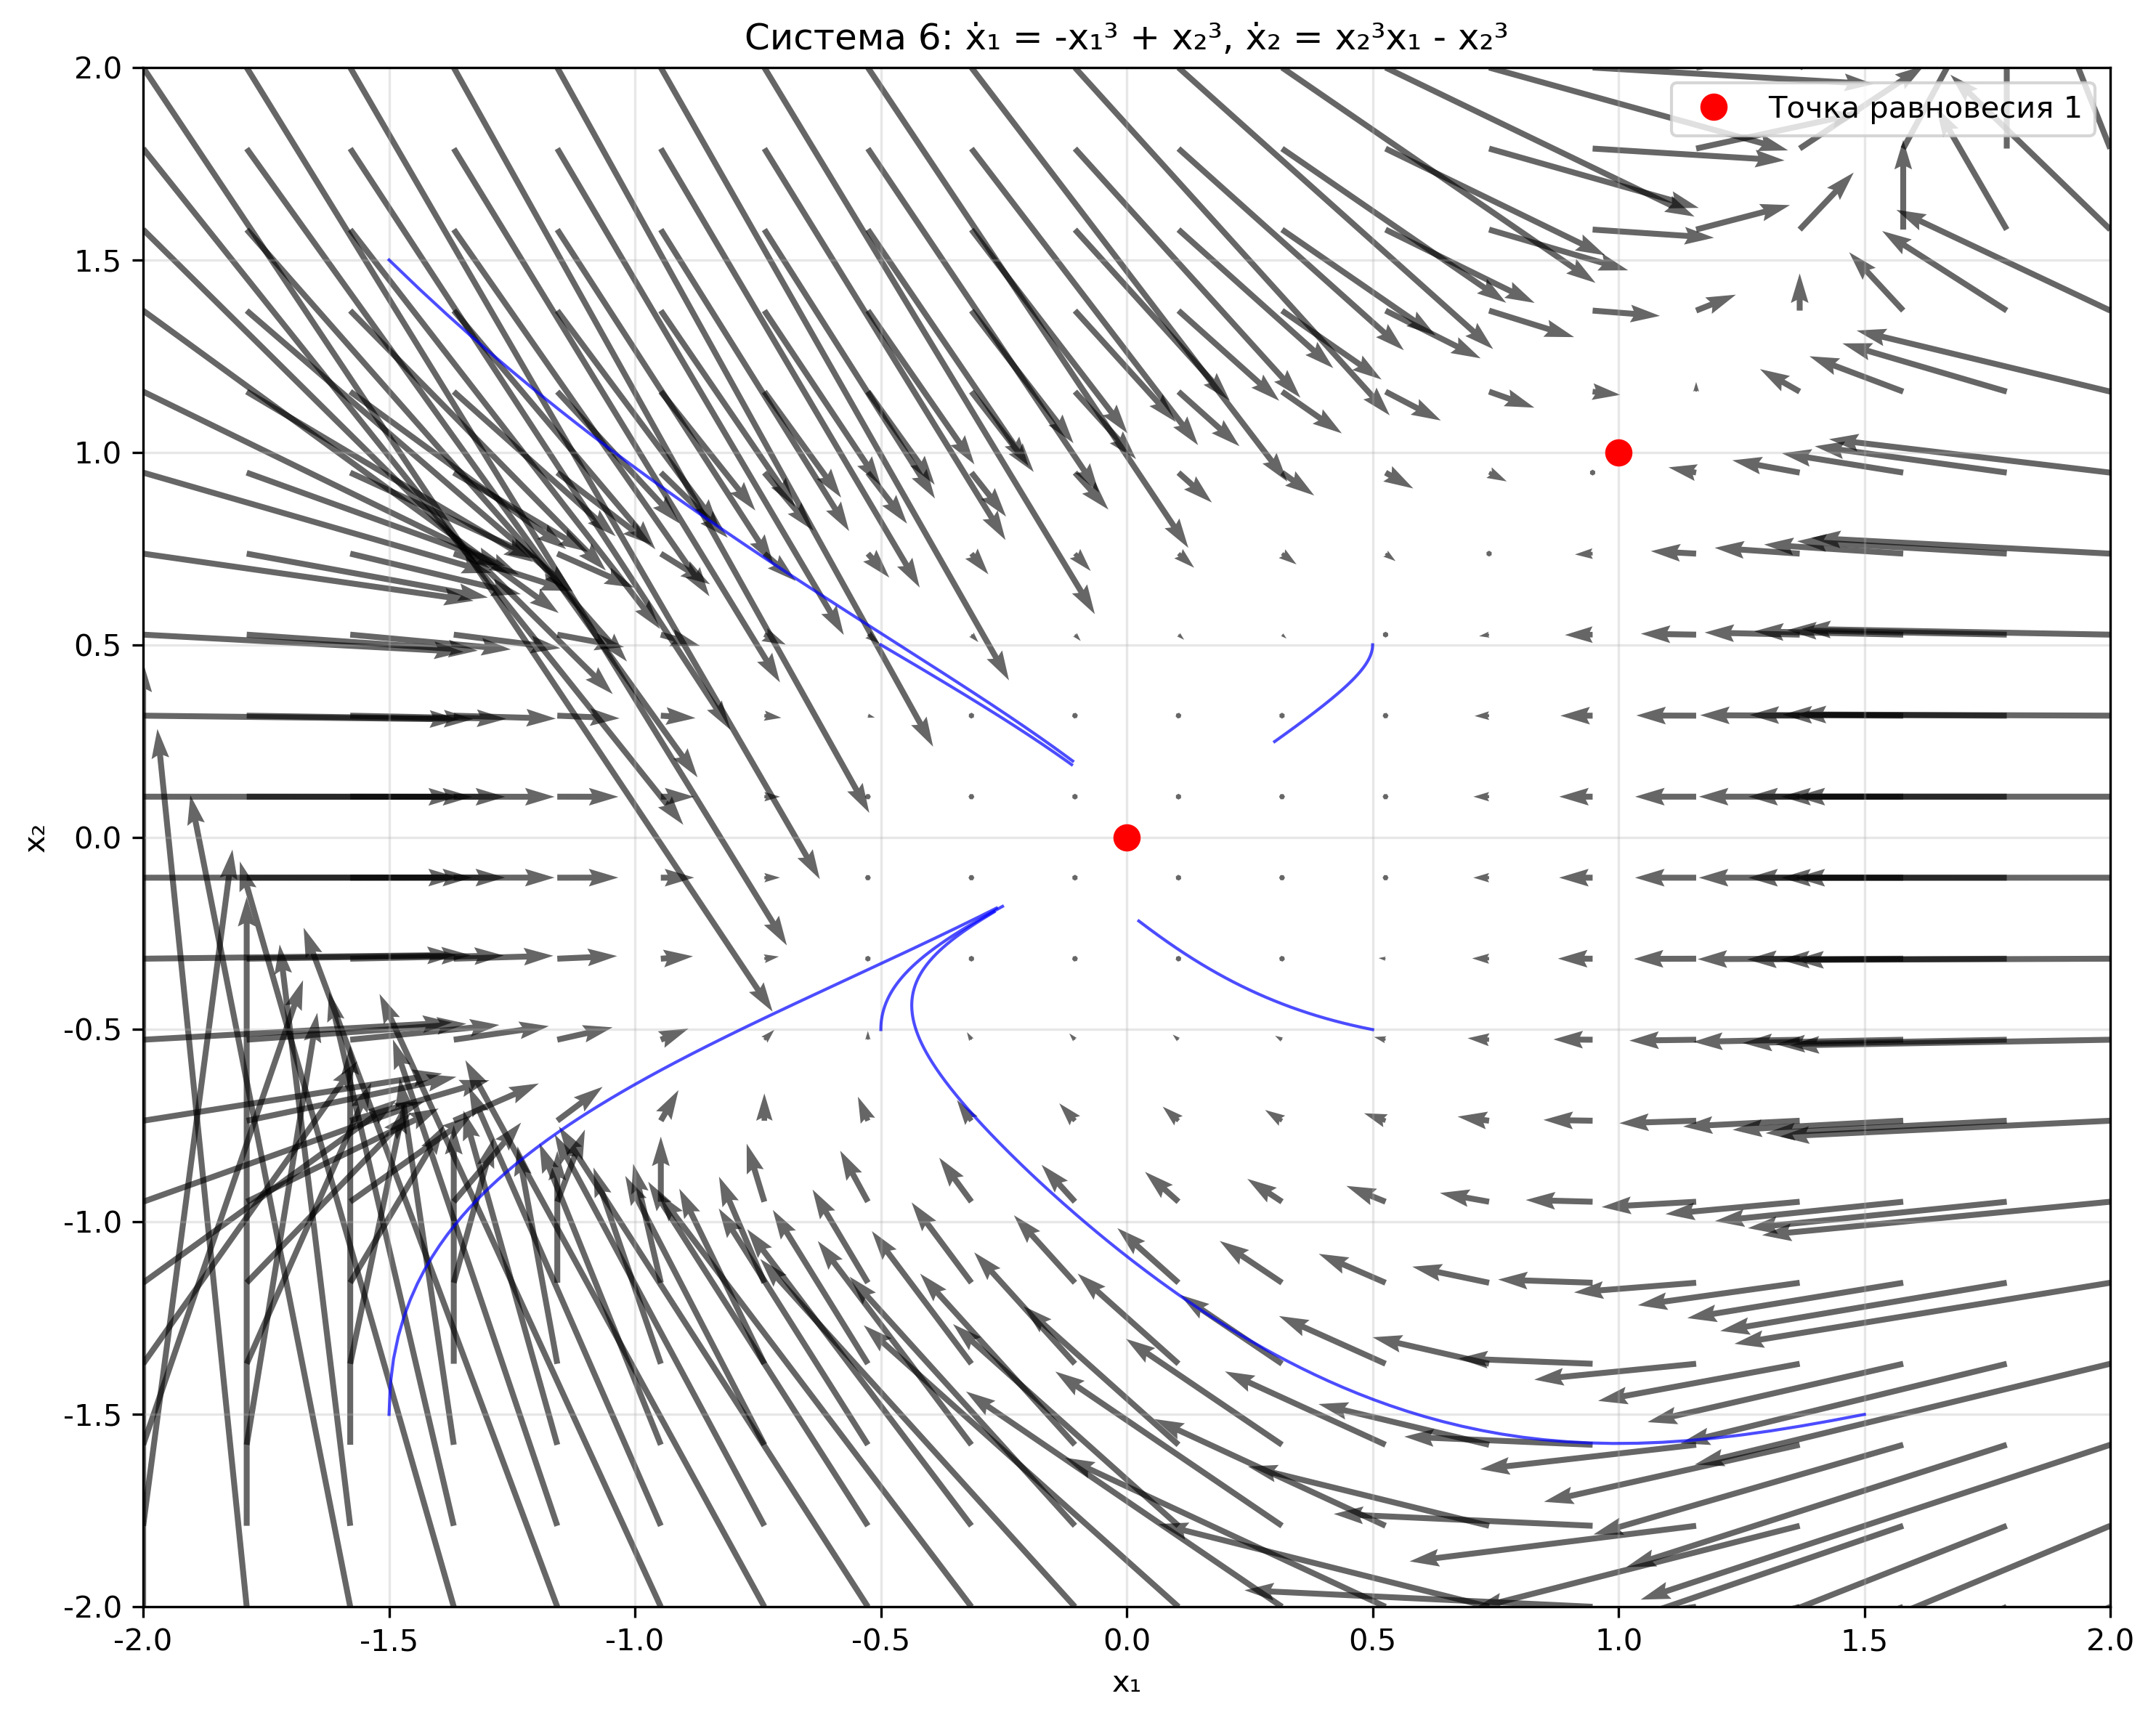
\includegraphics[width=0.8\textwidth]{phase_portraits/system6_phase_portrait.png}
\caption{Фазовый портрет системы 6}
\label{fig:system6_phase_portrait}
\end{figure}

\subsection*{Система 7}

\begin{align}
\dot{x}_1 &= -x_1^3 + x_2^3 \\
\dot{x}_2 &= x_1 + 3x_3 - x_2^3 \\
\dot{x}_3 &= x_1 x_3 - x_2^3 - \sin x_1
\end{align}

\textbf{Точки равновесия:}
\begin{align}
-x_1^3 + x_2^3 &= 0 \\
x_1 + 3x_3 - x_2^3 &= 0 \\
x_1 x_3 - x_2^3 - \sin x_1 &= 0
\end{align}

	extbf{Единственная точка равновесия:} $(0, 0, 0)$

Проверка:
\begin{itemize}
\item $f_1(0,0,0) = -0^3 + 0^3 = 0$ ✓
\item $f_2(0,0,0) = 0 + 3 \cdot 0 - 0^3 = 0$ ✓
\item $f_3(0,0,0) = 0 \cdot 0 - 0^3 - \sin(0) = 0$ ✓
\end{itemize}

\textbf{Матрица Якоби:}
$$J = \begin{pmatrix} 
-3x_1^2 & 3x_2^2 & 0 \\
1 & -3x_2^2 & 3 \\
x_3 - \cos x_1 & -3x_2^2 & x_1
\end{pmatrix}$$

\textbf{Анализ точки равновесия:}
В точке $(0, 0, 0)$:
$\lambda_1 = \lambda_2 = \lambda_3 = 0$ (тройной корень) --- вырожденный случай
Для системы 4 проведен анализ предельных циклов с использованием перехода к полярным координатам.


\begin{figure}[H]
\centering
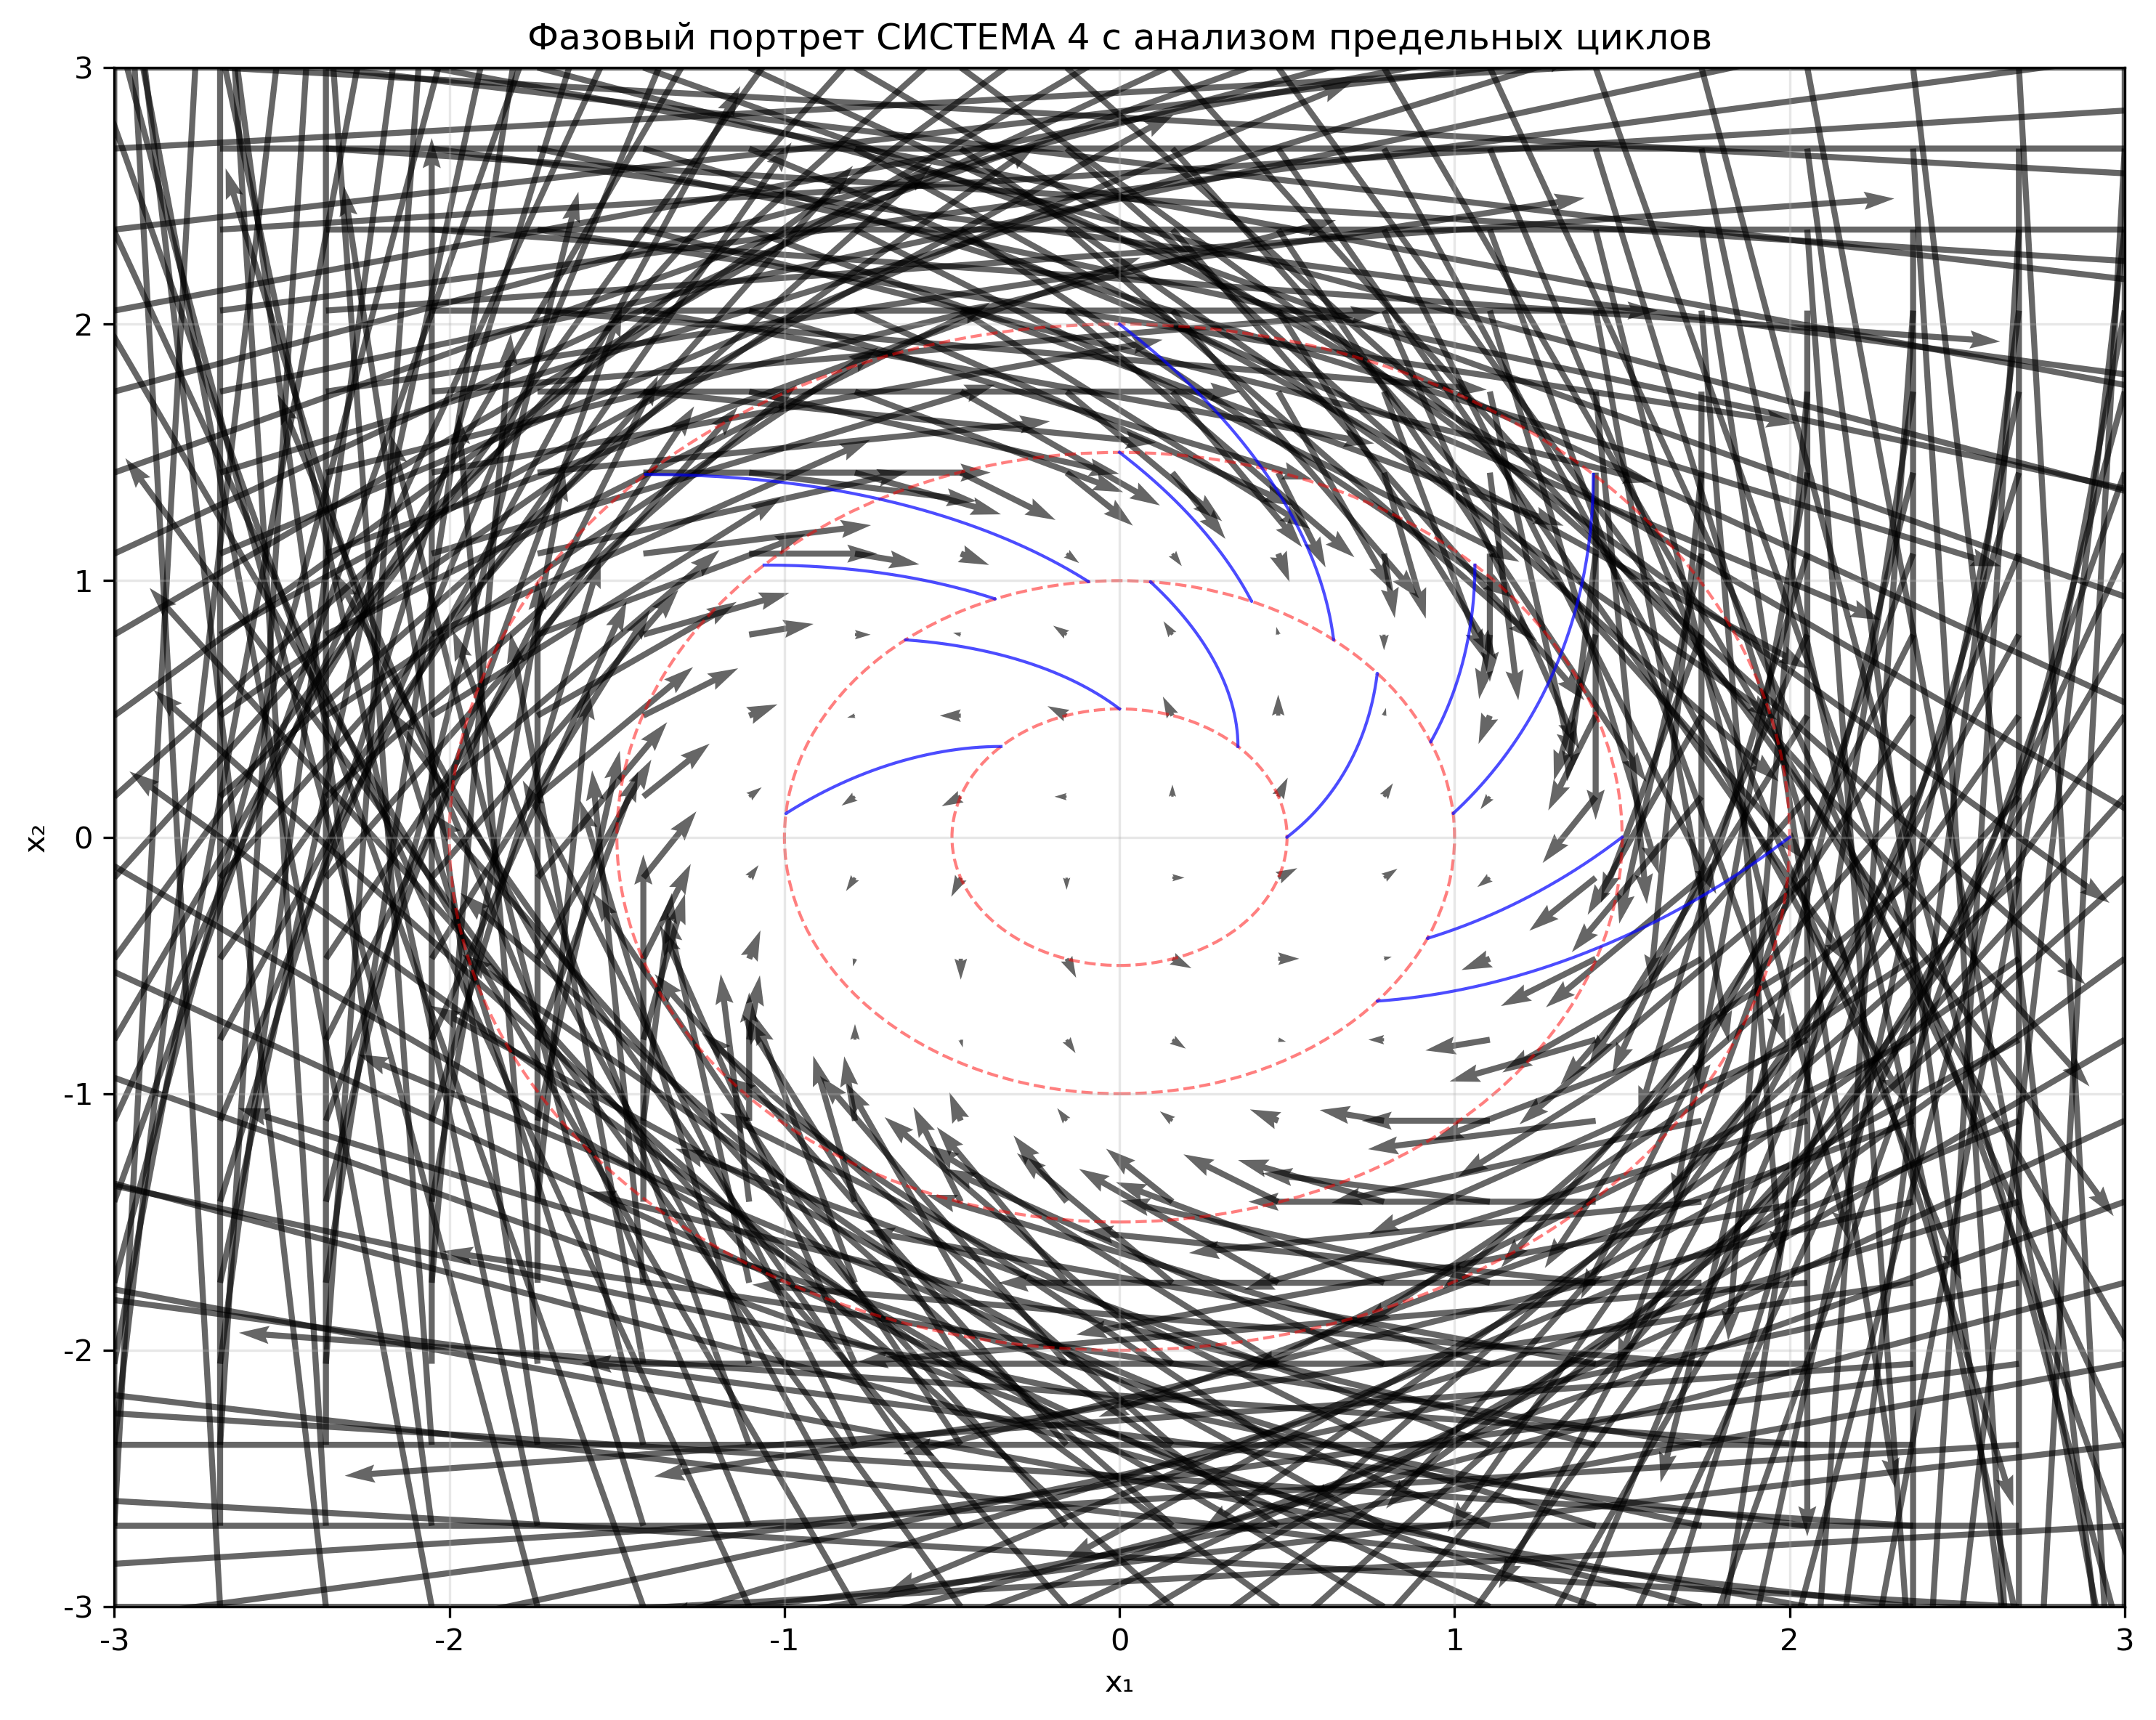
\includegraphics[width=0.8\textwidth]{limit_cycles/limit_cycles_система_4.png}
\caption{Фазовый портрет системы 4 с анализом предельных циклов}
\label{fig:limit_cycles_system4}
\end{figure}
